\documentclass[
	12pt,				
	openright,			
	oneside,			
	a4paper,			
	english,			
	brazil				
	]{abntex2}

\usepackage[utf8]{inputenc}
\usepackage[T1]{fontenc}
\usepackage{lmodern}
\usepackage{graphicx} 
\usepackage{amsmath}
\usepackage{amssymb}
\usepackage{indentfirst}
\usepackage{microtype}
\usepackage[alf]{abntex2cite}
\usepackage{xcolor}
\usepackage{tcolorbox}
\usepackage{booktabs}
\usepackage{caption}
\usepackage{ltablex}
\usepackage{svg}
\usepackage[left=3cm,right=2cm,top=3cm,bottom=2cm]{geometry}
\usepackage{tikz}
\usetikzlibrary{positioning, shapes.geometric, arrows.meta, fit, backgrounds}
\usepackage{url}
\usepackage{hyperref}

\definecolor{codebg}{HTML}{2E3440}   % Cor de fundo estilo terminal nórdico
\definecolor{codetext}{HTML}{ECEFF4} % Cor da fonte clara

\newtcolorbox{searchquery}{
    colback=codebg,      
    coltext=codetext,    
    colframe=codebg,     
    boxrule=0pt,         
    arc=3pt,             
    fontupper=\ttfamily\small, 
    left=6pt, right=6pt, top=4pt, bottom=4pt, 
    width=\linewidth,    
    nobeforeafter        
}

% --- Informações do Trabalho ---
\titulo{SOLUÇÃO PARA EXTRAÇÃO E CLASSIFICAÇÃO EM FATURAS DE CARTÃO DE CRÉDITO UTILIZANDO FERRAMENTAS DE INTELIGÊNCIA ARTIFICIAL}
\autor{Luiz Henrique Monteiro Silva Lima}
\local{Itaquaquecetuba, SP}
\data{2026}
\instituicao{Universidade de São Paulo -- USP \\ Instituto de Ciências Matemáticas e de Computação -- ICMC \\ MBA em Inteligência Artificial e Big Data}
\tipotrabalho{Monografia de Conclusão de Curso}
\preambulo{Monografia apresentada ao MBA em Inteligência Artificial e Big Data da Universidade de São Paulo (USP) como requisito parcial para a obtenção do título de Especialista.}

\begin{document}

% --- Elementos Pré-Textuais ---
\imprimircapa
\imprimirfolhaderosto

\pdfbookmark[0]{\listfigurename}{lof}
\listoffigures*
\cleardoublepage

\pdfbookmark[0]{\listtablename}{lot}
\listoftables*
\cleardoublepage

\pdfbookmark[0]{Lista de Abreviaturas e Siglas}{siglas}
\begin{siglas}
	\item[ABECS] Associação Brasileira das Empresas de Cartões de Crédito e Serviços
	\item[ABNT] Associação Brasileira de Normas Técnicas
	\item[API] Application Programming Interface
	\item[AUC] Area Under Curve
	\item[BERT] Bidirectional Encoder Representations from Transformers
	\item[BI] Business Intelligence
	\item[ByT5] Byte-level T5
	\item[CER] Character Error Rate (Taxa de Erro de Caracteres)
	\item[CNN] Convolutional Neural Network (Rede Neural Convolucional)
	\item[CPGF] Cartão de Pagamento do Governo Federal
	\item[CRISP-DM] Cross-Industry Standard Process for Data Mining
	\item[CT] Continuous Training (Treinamento Contínuo)
	\item[DLA] Document Layout Analysis (Análise de Layout de Documentos)
	\item[DVC] Data Version Control
	\item[FN] Falso Negativo
	\item[FP] Falso Positivo
	\item[GPU] Graphics Processing Unit
	\item[GRU] Gated Recurrent Unit
	\item[IAM] Identity and Access Management
	\item[IEEE] Institute of Electrical and Electronics Engineers
	\item[JSON] JavaScript Object Notation
	\item[KNN] K-Nearest Neighbors
	\item[LGPD] Lei Geral de Proteção de Dados Pessoais (Lei nº 13.709/2018)
	\item[LLM] Large Language Model (Grande Modelo de Linguagem)
	\item[LOR] Logarithmic Overfitting Ratio
	\item[LSTM] Long Short-Term Memory
	\item[MAE] Mean Absolute Error (Erro Absoluto Médio)
	\item[MCC] Matthews Correlation Coefficient
	\item[ML] Machine Learning (Aprendizado de Máquina)
	\item[MLflow] Machine Learning Flow (Plataforma de MLOps)
	\item[MLOps] Machine Learning Operations
	\item[MSE] Mean Squared Error (Erro Quadrático Médio)
	\item[NFE] Nota Fiscal Eletrônica
	\item[NLTK] Natural Language Toolkit
	\item[OCR] Optical Character Recognition (Reconhecimento Óptico de Caracteres)
	\item[OIDC] OpenID Connect
	\item[OOV] Out-Of-Vocabulary (Fora do Vocabulário)
	\item[PDF] Portable Document Format
	\item[PGVector] PostgreSQL Vector Extension
	\item[PLN] Processamento de Linguagem Natural
	\item[RAG] Retrieval-Augmented Generation
	\item[RAM] Random Access Memory
	\item[RBAC] Role-Based Access Control
	\item[Regex] Regular Expressions (Expressões Regulares)
	\item[REST] Representational State Transfer
	\item[RMSE] Root Mean Squared Error (Raiz do Erro Quadrático Médio)
	\item[RNN] Recurrent Neural Network (Rede Neural Recorrente)
	\item[ROC] Receiver Operating Characteristic
	\item[ROUGE] Recall-Oriented Understudy for Gisting Evaluation
	\item[S3] Simple Storage Service
	\item[SMOTE] Synthetic Minority Over-sampling Technique
	\item[SOTA] State-of-the-Art (Estado da Arte)
	\item[SPC] Serviço de Proteção ao Crédito
	\item[SQL] Structured Query Language
	\item[SVM] Support Vector Machines
	\item[TF-IDF] Term Frequency-Inverse Document Frequency
	\item[TN] Verdadeiro Negativo
	\item[TP] Verdadeiro Positivo
	\item[USP] Universidade de São Paulo
	\item[VRAM] Video Random Access Memory
	\item[WER] Word Error Rate (Taxa de Erro de Palavras)
	\item[XGBoost] Extreme Gradient Boosting
\end{siglas}
\cleardoublepage

\pdfbookmark[0]{\contentsname}{toc}
\tableofcontents*
\cleardoublepage

\textual

% ==============================================================================
% CAPÍTULO 1 - INTRODUÇÃO
% ==============================================================================
\chapter{Introdução}
\label{chp:introducao}

\section{Considerações Iniciais}
\label{sec:intro_consideracoes_iniciais}

O gerenciamento financeiro pessoal constitui uma das competências mais críticas e desafiadoras para os cidadãos no cenário econômico contemporâneo. Com a digitalização em massa dos meios de pagamento e a consequente substituição do dinheiro em espécie por instrumentos eletrônicos, o volume de dados transacionais gerados cotidianamente atingiu patamares sem precedentes. No entanto, o aumento na facilidade de transacionar não foi acompanhado por ferramentas automáticas eficazes de organização e inteligência orçamentária, gerando um descompasso estrutural entre o consumo e a visibilidade financeira dos indivíduos. Este capítulo contextualiza a problemática da despadronização de descrições em faturas de cartão de crédito, formaliza o problema de pesquisa, apresenta as motivações e justificativas deste trabalho, define os objetivos gerais e específicos, e detalha a organização estrutural desta monografia.

\section{Contextualização e Formulação do Problema}
\label{sec:intro_contextualizacao}

A popularização do cartão de crédito como o principal meio de pagamento no Brasil trouxe consigo um desafio crescente: a dificuldade de compreender e organizar os próprios gastos de forma autônoma e tempestiva. Segundo dados consolidados pela Associação Brasileira das Empresas de Cartões de Crédito e Serviços \cite{abecs2024panorama}, as compras realizadas com cartões de crédito, débito e pré-pagos movimentaram aproximadamente 4,1 trilhões de reais em 2024, evidenciando o papel central desses instrumentos na economia nacional. Paralelamente, dados divulgados pela Serasa Experian \cite{serasa2024inadimplencia} indicam a existência de mais de 200 milhões de cartões de crédito ativos no país, sendo que cerca de 29,37\% dos consumidores brasileiros inadimplentes possuíam dívidas diretamente vinculadas ao crédito rotativo ou ao parcelamento de faturas.

O crescimento no volume transacional é impulsionado tanto pelas compras em estabelecimentos físicos quanto pelo comércio eletrônico (\textit{e-commerce}). Relatórios de hábitos de consumo demonstram que os gastos digitais apresentaram expansão superior a 15\% ao final de 2024 \cite{poder360_2025}. Não obstante a conveniência proporcionada por essa digitalização, a falta de padronização nas informações repassadas aos usuários nas faturas mensais impede o planejamento consciente. Conforme apontado pelo Serviço de Proteção ao Crédito \cite{spcbrasil2024controle}, a grande maioria dos consumidores não possui um controle sistemático de seu orçamento mensal, recorrendo frequentemente a anotações manuais em planilhas ou cadernos — práticas propensas a erros e com altas taxas de abandono ao longo do tempo.

\begin{figure}[htb]
    \centering
    \caption{Exemplo ilustrativo de despadronização e ruídos em extrato de cartão de crédito.}
    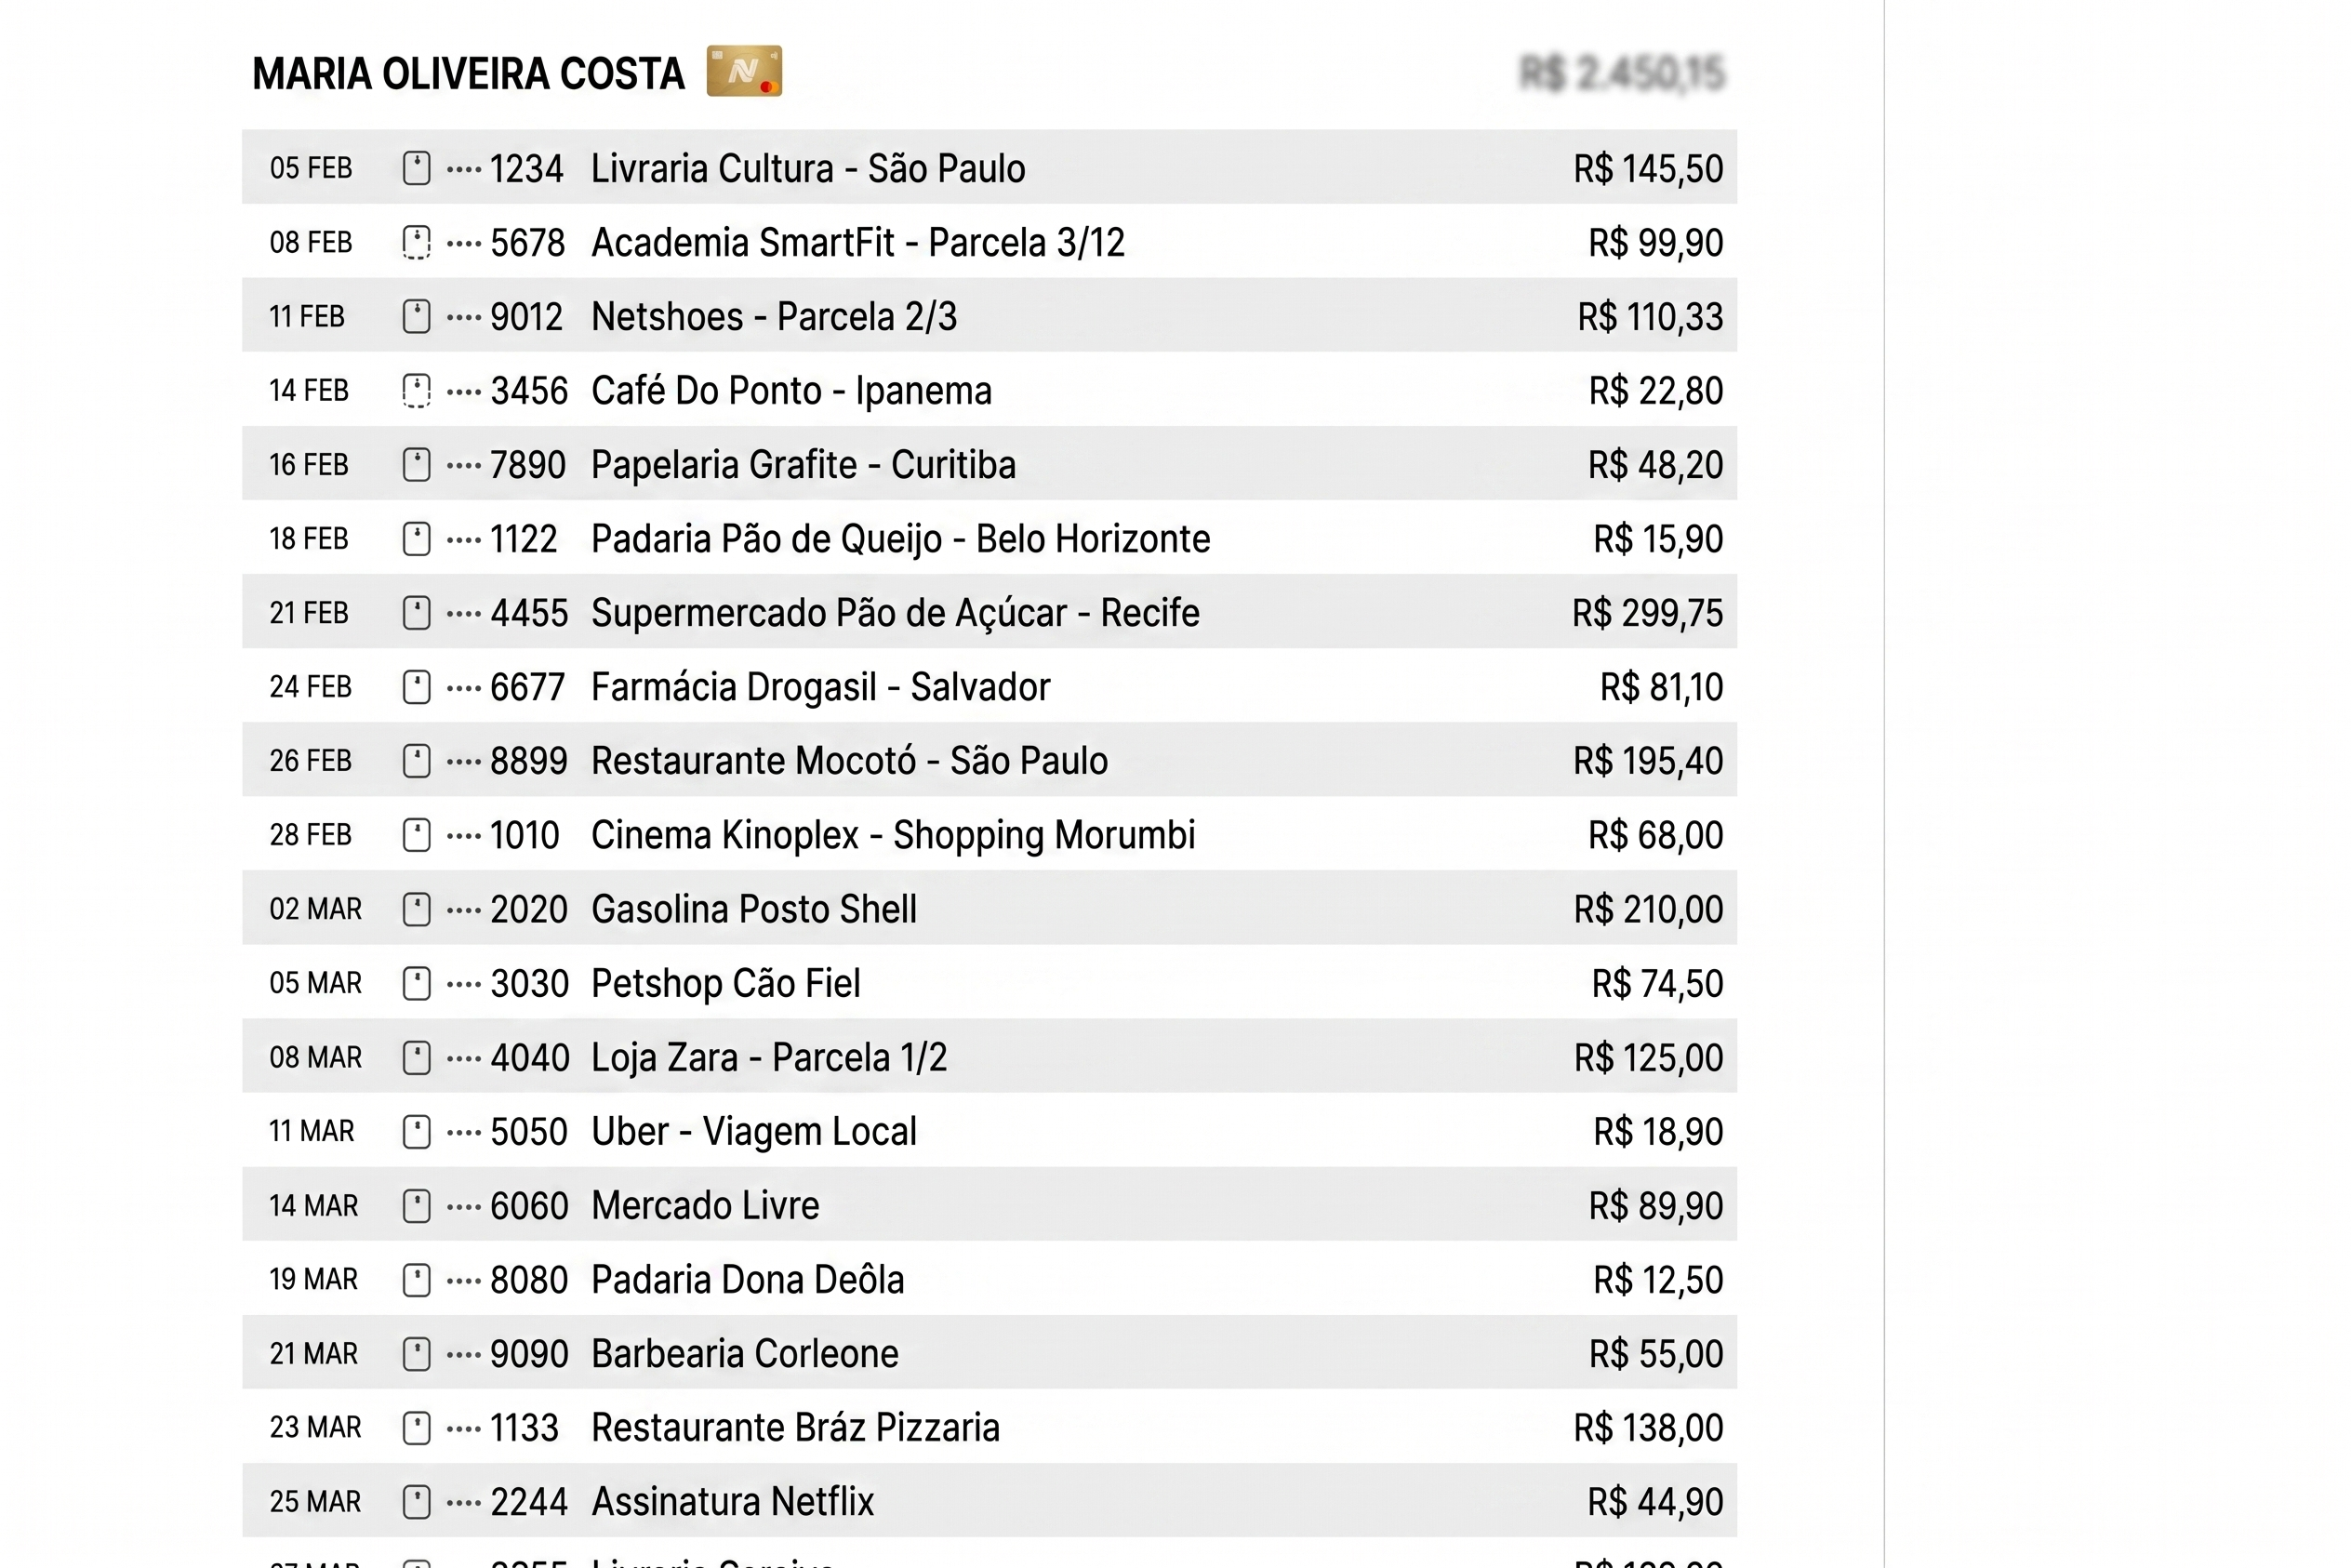
\includegraphics[width=0.88\textwidth]{assets/fatura_imaginaria.png}
    \label{fig:fatura_exemplo}
    \fonte{Elaborado pelo autor (\the\year).}
\end{figure}

O \textbf{problema central investigado nesta pesquisa} reside na \textbf{categorização automática, precisa e escalável de transações financeiras de cartão de crédito a partir de descrições textuais curtas, heterogêneas, ruidosas e altamente despadronizadas}. Conforme ilustrado na Figura~\ref{fig:fatura_exemplo}, as linhas de extrato apresentam obstáculos multidimensionais:
\begin{enumerate}
    \item \textbf{Abreviações e Siglas Crípticas:} Nomes de fornecedores frequentemente aparecem severamente truncados, concatenados ou representados por razões sociais obsoletas (ex.: ``AMZN MKTPLACE'', ``PAG*RestSaoPaulo'', ``DL*GOOGLE'');
    \item \textbf{Prefixos de Processadores e Gateways de Pagamento:} Transações intermediadas por terminais eletrônicos (maquininhas) e facilitadores digitais inserem códigos e prefixos alfanuméricos espúrios (ex.: ``PG*'', ``MP*'', ``ZOOP*'', ``SUMUP*'') que ocultam a identidade real do estabelecimento;
    \item \textbf{Ruídos Decorrentes de Leitura Óptica (OCR):} Em documentos digitalizados, escaneados ou fotografados por câmeras móveis, motores de Reconhecimento Óptico de Caracteres introduzem erros de substituição, deleção e inserção de caracteres (ex.: letras trocadas por números semelhantes), gerando palavras fora do vocabulário padrão (\textit{Out-Of-Vocabulary} -- OOV);
    \item \textbf{Ambiguidade de Marketplaces e Multicategorias:} Grandes plataformas de comércio eletrônico (como Mercado Livre, Amazon e Shopee) transacionam mercadorias de naturezas diametralmente opostas (eletrônicos, vestuário, alimentação, medicamentos) sob uma mesma fatura corporativa genérica, tornando a inferência categórica impossível apenas pelo texto bruto do canal;
    \item \textbf{Privacidade e Soberania dos Dados Financeiros:} O tratamento de dados transacionais bancários envolve informações de alta sensibilidade pessoal, exigindo estrita conformidade com a Lei Geral de Proteção de Dados Pessoais (LGPD -- Lei nº 13.709/2018) \cite{brasil2018lgpd}, o que restringe o envio indiscriminado de extratos a serviços terceirizados e APIs proprietárias em nuvem pública.
\end{enumerate}

\section{Motivação e Justificativa}
\label{sec:intro_motivacao}

A motivação deste trabalho apoia-se em duas perspectivas complementares: o avanço técnico-científico na área de Ciência da Computação e o impacto socioeconômico direto na gestão orçamentária dos cidadãos.

No âmbito da \textbf{Ciência da Computação}, o problema integra de maneira transdisciplinar a Visão Computacional/OCR, o Processamento de Linguagem Natural (PLN), os Sistemas de Recuperação de Informação Vetorial (RAG), a Engenharia de Agentes Inteligentes baseados em Grafos de Estado e as práticas de Operações de Aprendizado de Máquina (MLOps). Desenvolver uma arquitetura que funcione com alta precisão sob restrições severas de hardware local (sem demandar clusters de GPU de alto custo) preenche uma lacuna relevante na literatura de Inteligência Artificial aplicada, demonstrando a viabilidade de pipelines modulares, reativos e energeticamente eficientes.

Sob o ponto de vista \textbf{aplicado e socioeconômico}, automatizar o processo de saneamento e classificação de despesas elimina o esforço cognitivo e a sobrecarga de tempo associados à gestão financeira pessoal. Ao fornecer categorias precisas, justificativas semânticas inteligíveis e mecanismos de aprendizado contínuo com intervenção humana (\textit{Human-in-the-Loop}), o sistema capacita os usuários a compreender seus reais padrões de consumo, auxiliando na prevenção do endividamento precoce e promovendo a sustentabilidade orçamentária das famílias.

\section{Objetivos}
\label{sec:intro_objetivos}

O \textbf{objetivo geral} desta monografia é conceber, implementar e validar experimentalmente uma solução computacional de ponta a ponta baseada em ferramentas de Inteligência Artificial para a extração, normalização e classificação automática de transações financeiras em faturas de cartão de crédito, assegurando alta acurácia preditiva, resiliência a ruídos textuais e ópticos, privacidade dos dados e sustentabilidade operacional.

Para concretizar o objetivo geral, definiram-se os seguintes \textbf{objetivos específicos}:

\begin{enumerate}
    \item \textbf{Ingestão e Extração Híbrida de Documentos:} Desenvolver um módulo capaz de ingerir faturas em formatos digitais nativos (CSV, OFX, JSON) e documentos ópticos (PDFs digitalizados e imagens), combinando conversores avançados com análise de layout (\textit{Docling}) e motores de OCR locais (\textit{Tesseract}) com filtragem de confiança;
    \item \textbf{Pipeline de Normalização e Saneamento Léxico:} Projetar rotinas algorítmicas de pré-processamento para eliminação de prefixos de gateways de pagamento, supressão de ruídos alfanuméricos e resolução de sinônimos/aliases comerciais;
    \item \textbf{Estabelecimento de Linhas de Base Científicas (\textit{Baselines}):} Implementar e mensurar o desempenho de algoritmos de aprendizado de máquina clássico (Naive Bayes e Random Forest) acoplados à vetorização estatística TF-IDF, estabelecendo referências quantitativas de comparação;
    \item \textbf{Modelagem com Transformers e Recuperação Vetorial (RAG):} Construir uma base de conhecimento densa em banco de dados relacional e vetorial (\textit{PostgreSQL} com extensão \textit{pgvector}), permitindo buscas semânticas em milissegundos via embeddings multilíngues e investigando modelos no nível de byte/caractere (\textit{ByT5});
    \item \textbf{Arquitetura de Agente Inteligente com Grafos de Estado:} Orquestrar a tomada de decisão preditiva através de um grafo de estados (\textit{LangGraph}), integrando prompts dinâmicos conscientes da origem do dado, ferramentas autônomas de busca na web (\textit{DuckDuckGo}), estruturas Pydantic com cadeias de pensamento (\textit{Chain-of-Thought}) e pausas programadas para confirmação humana (\textit{Human-in-the-Loop}) em casos ambíguos;
    \item \textbf{Estruturação de Data Lakehouse e Esteira MLOps:} Desenvolver a infraestrutura conteinerizada da solução apoiada em armazenamento em camadas (MinIO Bronze/Silver), mensageria por eventos (Apache Kafka), rastreamento experimental e versionamento de modelos (MLflow);
    \item \textbf{Validação Experimental e Diagnóstico Comparativo:} Avaliar quantitativamente a acurácia, precisão, recall, F1-Score Macro, matriz de confusão e latência em conjuntos de dados reais e sintéticos contendo mais de 470 mil registros, verificando formalmente as hipóteses de pesquisa.
\end{enumerate}

\section{Organização da Monografia}
\label{sec:intro_organizacao}

O presente documento está estruturado em seis capítulos e dois apêndices, organizados de forma sequencial e lógica conforme descrito a seguir:

\begin{itemize}
    \item \textbf{Capítulo 1 -- Introdução:} Apresenta as considerações iniciais, a contextualização da pesquisa, a formalização do problema de faturas despadronizadas, as motivações técnica e socioeconômica, os objetivos geral e específicos, e a visão geral da estrutura do trabalho;
    \item \textbf{Capítulo 2 -- Fundamentação Teórica:} Discute os conceitos teóricos essenciais que sustentam a solução, abrangendo Processamento de Linguagem Natural, tokenização em subpalavras/bytes, modelos densos de embeddings, bancos de dados vetoriais, visão computacional e OCR, arquiteturas neurais Transformer, agentes inteligentes em grafos e práticas contemporâneas de MLOps e Data Lakehouse;
    \item \textbf{Capítulo 3 -- Trabalhos Relacionados:} Analisa o estado da arte por meio de uma revisão estruturada da literatura, confrontando estudos sobre saneamento pós-OCR, mineração de textos informais e extração em notas fiscais, sintetizados em um quadro comparativo que explicita as lacunas abordadas por esta pesquisa;
    \item \textbf{Capítulo 4 -- Solução Proposta:} Detalha a engenharia do sistema, formalizando as questões de pesquisa e a hipótese central, o framework metodológico CRISP-DM adaptado, a arquitetura de Data Lakehouse conteinerizada, o fluxo de extração híbrida, o grafo de estados do agente inteligente (LangGraph), as salvaguardas de privacidade e LGPD, e a estratégia de garantia de qualidade;
    \item \textbf{Capítulo 5 -- Validação Experimental e Resultados:} Expõe o ambiente computacional, a caracterização dos datasets utilizados (CPGF, faturas reais de bancos digitais e dados com ruídos sintéticos), o protocolo de avaliação, as métricas obtidas nos baselines clássicos versus agente híbrido, as análises de ablação e a verificação formal das hipóteses;
    \item \textbf{Capítulo 6 -- Conclusões e Trabalhos Futuros:} Sintetiza as principais contribuições técnicas alcançadas, avalia o cumprimento dos objetivos, discute as limitações identificadas e aponta direções para continuidade e evolução da pesquisa em cenários como Open Finance e aprendizado federado;
    \item \textbf{Apêndices:} O Apêndice A apresenta o protocolo detalhado do levantamento bibliográfico (strings booleanas, bases de dados e critérios de triagem), e o Apêndice B expõe o esquema do banco de dados relacional e vetorial implementado.
\end{itemize}

% ==============================================================================
% CAPÍTULO 2 - FUNDAMENTAÇÃO TEÓRICA
% ==============================================================================
\chapter{Fundamentação Teórica}
\label{chp:fundamentacao}

\section{Considerações Iniciais}
\label{sec:fund_consideracoes_iniciais}

A concepção de uma ferramenta robusta para a interpretação e categorização de faturas financeiras requer o domínio integrado de fundamentos oriundos de múltiplas subáreas da Inteligência Artificial e da Engenharia de Software. Este capítulo estabelece as bases conceituais estritamente instrumentais ao projeto, organizando-se em quatro pilares fundamentais: (i) Mineração de Textos e Processamento de Linguagem Natural; (ii) Visão Computacional, Análise de Layout e Reconhecimento Óptico de Caracteres (OCR); (iii) Arquiteturas Neurais Profundas e Agentes Inteligentes baseados em Grafos; e (iv) Engenharia de Dados, MLOps e Sustentabilidade de Modelos em Produção.

\section{Mineração de Textos e Processamento de Linguagem Natural}
\label{sec:fund_pln}

O Processamento de Linguagem Natural (PLN) constitui o ramo da Inteligência Artificial dedicado a capacitar sistemas computacionais a compreender, interpretar, manipular e gerar linguagens humanas \cite{BPLN_livro:2024, chowdhury2003natural}. No domínio financeiro, o desafio central da mineração textual reside na natureza não estruturada e altamente degenerada das descrições de compras em cartões de crédito \cite{santos2023classificacao}.

\subsection{Pré-processamento Léxico e Morfológico}
A primeira barreira técnica na modelagem de textos curtos é a dispersão léxica. A padronização morfológica atua reduzindo a alta dimensionalidade do vocabulário através de operações determinísticas \cite{BPLN_livro:2024}: conversão para caixa baixa (\textit{lowercasing}), normalização de caracteres acentuados via codificação Unicode e aplicação de Expressões Regulares (Regex) para supressão de pontuações, caracteres de controle e símbolos especiais.

Adicionalmente, a literatura enfatiza a remoção de \textit{stopwords} — palavras de alta frequência sem valor semântico discriminativo (artigos, preposições, conjunções) \cite{matos2010pre}. Contudo, listas genéricas universais mostram-se insuficientes no domínio financeiro. É mandatório injetar heurísticas específicas do negócio para remover sufixos de naturezas jurídicas e corporativas (como ``LTDA'', ``S/A'', ``ME'', ``EPP'', ``EIRELI'') e prefixos de liquidação financeira (``COMPRA'', ``PARCELA'', ``DEBITO''), os quais atuam como ruídos que distorcem as distribuições estatísticas \cite{santos2023classificacao}.

\subsection{Estratégias de Tokenização: Da Palavra ao Nível de Byte}
A tokenização segmenta a cadeia textual contínua em unidades atômicas de processamento denominadas \textit{tokens} \cite{BPLN_livro:2024}. Modelos tradicionais baseados em palavras inteiras (\textit{word-level}) dependem de vocabulários fechados predefinidos. Diante de faturas financeiras, onde erros de digitação, truncamentos e aglutinações são onipresentes, essa abordagem falha sistematicamente devido à explosão de termos fora do vocabulário (\textit{Out-Of-Vocabulary} -- OOV).

Para superar essa fragilidade, o estado da arte avançou para a tokenização em subpalavras (\textit{subwords}, como Byte-Pair Encoding e WordPiece) e, no limite da granularidade, para a tokenização no nível de caractere ou byte \cite{xue2021byt5, zhang2021mineracao}. Modelos que operam diretamente sobre sequências de bytes UTF-8, a exemplo do ByT5 \cite{xue2021byt5}, eliminam completamente o vocabulário fixo. Essa característica confere ao sistema imunidade contra erros ortográficos e capacidade inata de generalizar sobre siglas desconhecidas e nomes comerciais aglutinados (ex.: ``MERCADOPAG*LOJA123'').

\subsection{Vetorização Estatística versus Representações Densas (Embeddings)}
Para que algoritmos computacionais processem dados textuais, é imperativo convertê-los em representações numéricas vetoriais.

\subsubsection{TF-IDF (Term Frequency-Inverse Document Frequency)}
A técnica clássica de TF-IDF quantifica a importância de um termo $t$ em um documento $d$ pertencente a um corpus $D$, calculada pelo produto da frequência do termo ($TF$) pelo inverso da frequência no documento ($IDF$) \cite{rajaraman2011mining}:
\begin{equation}
    \text{TF-IDF}(t, d, D) = \text{TF}(t, d) \times \log\left(\frac{|D|}{1 + |\{d \in D : t \in d\}|}\right)
\end{equation}
Embora gere matrizes esparsas de alta dimensionalidade que desconsideram o contexto e a ordem sintagmática das palavras, o TF-IDF permanece relevante como uma linha de base científica (\textit{baseline}) de referência rápida, interpretável e de baixo custo computacional \cite{santos2023classificacao}.

\subsubsection{Embeddings Densos e Bancos de Dados Vetoriais}
A superação das limitações esparsas consolidou-se com a semântica distribucional profunda. Modelos como o Sentence-BERT (SBERT) \cite{reimers2019sentence}, implementados através de arquiteturas siamesas de Sentence Transformers (ex.: \texttt{paraphrase-multilingual-MiniLM-L12-v2}), mapeiam sentenças inteiras em vetores densos e contínuos de dimensionalidade fixa (ex.: 384 dimensões).

Nesse espaço vetorial contínuo, a proximidade semântica entre duas transações $u$ e $v$ é mensurada diretamente pela similaridade de cosseno:
\begin{equation}
    \text{Simil}(u, v) = \frac{u \cdot v}{\|u\|_2 \|v\|_2} = \frac{\sum_{i=1}^{n} u_i v_i}{\sqrt{\sum_{i=1}^{n} u_i^2} \sqrt{\sum_{i=1}^{n} v_i^2}}
\end{equation}
Para viabilizar consultas em milissegundos sobre milhões de registros históricos, utilizam-se extensões vetoriais integradas ao banco de dados relacional, destacando-se a extensão \textit{pgvector} para PostgreSQL. Essa infraestrutura permite implementar mecanismos de Geração Aumentada por Recuperação (\textit{Retrieval-Augmented Generation} -- RAG), onde exemplos canônicos rotulados são recuperados dinamicamente para subsidiar a tomada de decisão do classificador.

\section{Visão Computacional e Inteligência de Documentos}
\label{sec:fund_visao_ocr}

A Inteligência de Documentos (\textit{Document AI}) integra Visão Computacional e PLN para extrair informações estruturadas de imagens e documentos não nativos \cite{docling2024}.

\subsection{Análise de Layout de Documentos (DLA) e Caixas Delimitadoras}
A Análise de Layout de Documentos (DLA) é a etapa encarregada de segmentar a imagem da página, identificando blocos lógicos como tabelas, colunas, parágrafos e cabeçalhos. Cada entidade visual é mapeada por coordenadas espaciais denominadas caixas delimitadoras (\textit{bounding boxes}): $[x_{\min}, y_{\min}, x_{\max}, y_{\max}]$.

Em faturas de cartão de crédito, a preservação da topologia e da ordem de leitura é mandatória: a relação espacial de alinhamento horizontal entre o nome do estabelecimento comercial e o seu respectivo valor monetário em reais (R\$) carrega a semântica relacional necessária para isolar a transação e evitar a fusão indevida de dados entre colunas paralelas \cite{drumond2023analise}.

\subsection{Motores de OCR e Ferramentas de Conversão Estruturada}
\begin{itemize}
    \item \textbf{Tesseract OCR:} Mecanismo de reconhecimento óptico de código aberto amplamente utilizado \cite{smith2007overview}. Baseia-se em redes neurais LSTM para converter matrizes de pixels em caracteres. O Tesseract opera localmente garantindo total privacidade, mas exige imagens rigorosamente limpas para evitar quedas acentuadas de precisão diante de ruídos visuais;
    \item \textbf{IBM Docling:} Ferramenta moderna de processamento documental (\textit{Document Parsing}) especializada na extração estruturada de PDFs complexos \cite{docling2024}. Ao combinar modelos de visão para segmentação de tabelas com exportação nativa em Markdown estruturado, o Docling preserva as linhas de transações tabulares sem depender de heurísticas frágeis de coordenadas manuais.
\end{itemize}

\subsection{Métricas Formais de Avaliação de OCR: CER e WER}
A qualidade da extração óptica é avaliada formalmente pela distância de edição de Levenshtein entre o texto predito pelo OCR e o texto de referência (\textit{ground truth}). Definem-se três tipos fundamentais de erro: Substituição ($S$), Deleção ($D$) e Inserção ($I$).

A \textbf{Taxa de Erro de Caracteres} (CER -- \textit{Character Error Rate}) é calculada sobre o total de caracteres de referência $N_c$:
\begin{equation}
    \text{CER} = \frac{S_c + D_c + I_c}{N_c}
\end{equation}

A \textbf{Taxa de Erro de Palavras} (WER -- \textit{Word Error Rate}) opera de forma idêntica, porém adotando palavras inteiras como unidade amostral sobre o total de palavras $N_w$:
\begin{equation}
    \text{WER} = \frac{S_w + D_w + I_w}{N_w}
\end{equation}
Um único caractere lido incorretamente invalida a palavra inteira no cálculo do WER, tornando esta métrica estritamente mais rigorosa que o CER \cite{araujo2024saneamento}.

\section{Arquiteturas Neurais e Agentes Inteligentes}
\label{sec:fund_arquiteturas_agentes}

\subsection{Mecanismos de Autoatenção e Arquiteturas Transformer}
A introdução do mecanismo de autoatenção (\textit{self-attention}) na arquitetura Transformer por Vaswani et al. \cite{vaswani2017attention} superou as limitações de paralelização das redes recorrentes tradicionais (LSTM e GRU) \cite{hochreiter1997long, cho2014learning}. A atenção escalada por produto escalar calcula o alinhamento contextual entre matrizes de Consulta ($Q$), Chave ($K$) e Valor ($V$):
\begin{equation}
    \text{Attention}(Q, K, V) = \text{softmax}\left(\frac{QK^T}{\sqrt{d_k}}\right)V
\end{equation}
Essa formulação permite que cada token pondere dinamicamente todos os demais elementos da sequência de entrada, capturando dependências semânticas não locais em textos curtos e informais.

\subsection{Grandes Modelos de Linguagem (LLMs) e Raciocínio Estruturado}
Os Grandes Modelos de Linguagem (\textit{Large Language Models} -- LLMs) pré-treinados em escala massiva demonstraram notável capacidade de inferência semântica e raciocínio contextual. Para mitigar o risco de alucinações e garantir o determinismo necessário a sistemas financeiros, duas técnicas são essenciais:
\begin{itemize}
    \item \textbf{Cadeia de Pensamento (\textit{Chain-of-Thought} -- CoT):} Induz o modelo a explicitar seus passos intermediários de raciocínio antes de emitir o veredito final, elevando comprovadamente a precisão lógica;
    \item \textbf{Chamada de Ferramentas (\textit{Tool Calling}):} Capacidade do modelo de suspender temporariamente a geração de texto para invocar funções externas (como motores de busca na web) a fim de obter evidências factuais em tempo real;
    \item \textbf{Saída Estruturada com Validação de Tipos:} Utilização de bibliotecas de validação de esquemas (como Pydantic) para forçar o modelo a responder exclusivamente em formatos JSON estritos e tipados.
\end{itemize}

\subsection{Orquestração Baseada em Grafos de Estado: LangGraph}
Enquanto cadeias lineares simples (\textit{chains}) são rígidas, aplicações complexas demandam arquiteturas cíclicas e com controle fino de fluxo. O \textit{LangGraph} \cite{langchain2024langgraph} estrutura a aplicação como um Grafo Direcionado de Estados (\textit{StateGraph}), onde cada nó executa uma função atômica (normalização, consulta vetorial, inferência LLM, persistência) e as arestas condicionais determinam o próximo passo baseando-se no estado tipado (\textit{AgentState}). O framework suporta nativamente persistência de memória (\textit{checkpoints}) e o padrão \textit{Human-in-the-Loop}, permitindo interromper o grafo de forma transparente para aguardar a confirmação humana e retomá-lo posteriormente.

\section{Engenharia de Dados, MLOps e Sustentabilidade de Modelos}
\label{sec:fund_mlops}

A sustentabilidade de uma solução de IA em ambientes de produção exige a incorporação de práticas de Engenharia de Dados e Operações de Aprendizado de Máquina (\textit{Machine Learning Operations} -- MLOps) \cite{kreuzberger2022mlops, treveil2020mlops}.

\subsection{Desvios Estatísticos: Data Drift e Concept Drift}
Modelos de machine learning operando sobre dados financeiros sofrem inevitável degradação temporal decorrente de dois fenômenos \cite{quinonero2008dataset, Lu2019LearningConceptDriftReview}:
\begin{itemize}
    \item \textbf{Data Drift (Desvio de Covariáveis):} Ocorre quando a distribuição das variáveis de entrada $P(X)$ se altera ao longo do tempo (ex.: novos nomes de estabelecimentos no mercado, atualização de gateways ou mudanças de formatação no OCR), embora a relação mapeada $P(Y|X)$ permaneça estável;
    \item \textbf{Concept Drift (Desvio de Conceito):} Manifesta-se quando a probabilidade condicional real $P(Y|X)$ muda (ex.: uma grande rede de postos de combustível que passa a atuar predominantemente como loja de conveniência/alimentação, alterando a categoria esperada para uma mesma descrição textual).
\end{itemize}

\subsection{Aprendizado Ativo (Active Learning) e Confident Learning}
Para contornar o custo proibitivo da rotulação manual exaustiva diante do surgimento contínuo de novas empresas, a literatura preconiza o Aprendizado Ativo (\textit{Active Learning}) \cite{ren2021aprendizagem}. Ao invés de amostrar dados aleatoriamente, o sistema calcula a incerteza estatística de suas inferências. Transações com escore de confiança inferior a um limiar seguro (ex.: confiança $\le 0.70$) são isoladas e encaminhadas para curadoria humana (\textit{Human-in-the-Loop}) \cite{northcutt2021aprendizagem}. Os dados confirmados expandem a base de conhecimento de forma cirúrgica e de alto valor agregado.

\subsection{Arquitetura de Data Lakehouse e Rastreamento com MLflow}
A infraestrutura de suporte a dados moderna adota o paradigma de Data Lakehouse, combinando a flexibilidade e o baixo custo de armazenamento de objetos compatíveis com S3 (como o MinIO) com as garantias transacionais e a organização em camadas (\textit{Medallion Architecture}) \cite{treveil2020mlops}:
\begin{itemize}
    \item \textbf{Camada Bronze:} Armazena os dados brutos e imutáveis exatamente como foram ingeridos (PDFs originais, extratos bancários em CSV, textos ruidosos extraídos);
    \item \textbf{Camada Silver:} Contém os dados limpos, saneados, normalizados e enriquecidos em esquemas analíticos (Parquet/Iceberg);
    \item \textbf{Camada Gold:} Tabelas agregadas e visões analíticas prontas para consumo por motores SQL distribuídos (Trino) e dashboards de inteligência de negócios (Metabase).
\end{itemize}

O ciclo de vida experimental e operacional é unificado pelo \textit{MLflow} \cite{treveil2020mlops}. A plataforma atua como repositório centralizado de parâmetros, métricas e artefatos, suportando execuções aninhadas (\textit{nested runs}) que viabilizam o rastreamento em dois níveis de granularidade: a corrida global correspondente à fatura completa e corridas filhas isoladas para cada transação individualmente classificada.

\section{Considerações Finais do Capítulo}
\label{sec:fund_consideracoes_finais}

Os conceitos apresentados neste capítulo constituem a fundamentação técnica indispensável para a construção da solução proposta. A integração entre normalização morfológica, embeddings densos no PostgreSQL com pgvector, análise de layout com Docling, orquestração em grafos com LangGraph e práticas contínuas de MLOps no Data Lakehouse estabelece um arcabouço metodológico sólido para solucionar o desafio de classificar faturas de cartão de crédito com alto desempenho e sobriedade computacional.

% ==============================================================================
% CAPÍTULO 3 - TRABALHOS RELACIONADOS
% ==============================================================================
\chapter{Trabalhos Relacionados}
\label{chp:trabalhos_relacionados}

\section{Considerações Iniciais}
\label{sec:rel_consideracoes_iniciais}

A identificação das lacunas de pesquisa e o delineamento das escolhas arquiteturais deste trabalho exigem uma análise rigorosa do estado da arte. Este capítulo sintetiza a literatura recente referente à extração, saneamento de erros ópticos e classificação de documentos comerciais e textos informais. O protocolo metodológico completo do levantamento bibliográfico (strings de busca booleanas, bases científicas consultadas e critérios de triagem) encontra-se formalizado no Apêndice~\ref{apendice:protocolo_busca}. Nas seções seguintes, apresentam-se a discussão crítica dos estudos selecionados, o quadro comparativo e o posicionamento distintivo da presente monografia.

\section{Levantamento Bibliográfico e Categorização dos Estudos}
\label{sec:rel_levantamento}

O levantamento bibliográfico foi conduzido nas principais bases indexadoras internacionais e nacionais (Scopus, IEEE Xplore, Web of Science e Google Scholar), cobrindo publicações entre 2016 e 2025. Os trabalhos recuperados dividem-se em duas categorias conceituais:
\begin{itemize}
    \item \textbf{Trabalhos Fortemente Relacionados:} Pesquisas dedicadas especificamente ao processamento de notas fiscais, faturas comerciais e saneamento de textos financeiros curtos oriundos de OCR;
    \item \textbf{Trabalhos Fracamente Relacionados:} Estudos focados em problemas afins, como mineração de textos informais em redes sociais, arquiteturas teóricas de autoatenção e classificação de layout baseada exclusivamente em visão computacional.
\end{itemize}

\section{Análise Crítica dos Estudos Selecionados}
\label{sec:rel_analise_estudos}

A seguir, examinam-se individualmente os trabalhos que compõem o núcleo do estado da arte, padronizados conforme seus objetivos, abordagem metodológica, validação experimental e principais conclusões.

\subsection{Dhingra et al. (2016) e Zhang et al. (2021)}
\textbf{Objetivo:} Investigar métodos de representação vetorial e classificação profunda em textos curtos, informais e altamente ruidosos provenientes de plataformas digitais e registros transacionais.

\textbf{Abordagem:} Os autores propuseram arquiteturas de Redes Neurais Recorrentes bidirecionais (Bi-GRU e LSTM) operando no nível de caracteres (\textit{character-level}), a exemplo do modelo \textit{tweet2vec} \cite{dhingra2016tweet2vec, zhang2021mineracao}. A abordagem constrói representações semânticas densas a partir de sequências de letras adjacentes sem depender de vocabulários fechados.

\textbf{Validação e Resultados:} A validação foi conduzida em corpora de mensagens curtas com gírias e erros ortográficos. Os resultados comprovaram a superioridade estatística da modelagem por caracteres sobre métodos tradicionais (como Bag-of-Words e TF-IDF), mitigando drasticamente a falha diante de palavras fora do vocabulário (\textit{Out-Of-Vocabulary}). 

\textbf{Relação com esta Pesquisa:} Fundamenta teoricamente a necessidade de decompor termos financeiros em subpalavras e caracteres para reconhecer descrições truncadas (ex.: ``IFD*RESTAUR'') que não constam em dicionários formais.

\subsection{Participantes da Competição ICDAR (2019) e Modelo CCC}
\textbf{Objetivo:} Promover o avanço de técnicas automatizadas para a extração de entidades e correção de erros de leitura óptica em recibos comerciais digitalizados (\textit{shopping receipts}) \cite{icdar2019competition}.

\textbf{Abordagem:} As equipes vencedoras do torneio internacional (com destaque para a arquitetura CCC) modelaram o saneamento pós-OCR como uma tarefa de tradução ponta a ponta (\textit{Sequence-to-Sequence}), acoplando codificadores baseados em BERT \cite{devlin2019bert} a camadas convolucionais para detecção e correção cirúrgica de caracteres corrompidos.

\textbf{Validação e Resultados:} Avaliados sobre milhares de cupons fiscais reais com distorções físicas e manchas de impressão, os modelos Transformer obtiveram reduções expressivas nas taxas de erro de caracteres (CER), superando abordagens determinísticas baseadas em regras de substituição manual.

\textbf{Relação com esta Pesquisa:} Comprova que a higienização de faturas e recibos deve ser tratada como tradução contextual texto-a-texto, evidenciando, contudo, que modelos massivos demandam infraestrutura de hardware custosa, o que justifica a investigação de modelos compactos nesta monografia.

\subsection{Santos (2023)}
\textbf{Objetivo:} Avaliar a viabilidade de algoritmos de aprendizado de máquina para classificar produtos em Notas Fiscais Eletrônicas (NFE) a partir de descrições textuais desestruturadas e curtas \cite{santos2023classificacao}.

\textbf{Abordagem:} O autor comparou um classificador clássico baseado em vetorização TF-IDF associada a algoritmos tradicionais contra uma Rede Neural Recorrente (LSTM) no nível de caracteres, treinadas para categorizar itens mercadológicos.

\textbf{Validação e Resultados:} A validação em dados reais de notas fiscais confirmou que a abordagem no nível de caracteres obteve ganhos expressivos de acurácia sobre o baseline clássico. Todavia, o estudo reportou dificuldades computacionais no treinamento sequencial de RNNs em máquinas convencionais e severa degradação preditiva nas classes minoritárias devido ao desbalanceamento extremo da base.

\textbf{Relação com esta Pesquisa:} Reforça a importância do processamento granular e demonstra a necessidade de adotar métricas robustas (como o F1-Score Macro) e arquiteturas baseadas em Transformers paralelizáveis e RAG para contornar o gargalo das classes desbalanceadas.

\subsection{Araújo et al. (2024)}
\textbf{Objetivo:} Avaliar comparativamente o desempenho e a eficiência computacional de modelos de linguagem compactos baseados em subpalavras contra Grandes Modelos de Linguagem (LLMs massivos) na tarefa de correção ortográfica Pós-OCR em textos curtos com ruído severo \cite{araujo2024saneamento}.

\textbf{Abordagem:} Os pesquisadores conduziram um estudo empírico confrontando modelos especializados e leves (ByT5 e BART) \cite{xue2021byt5, lewis2020bart} com modelos generativos bilionários (LLaMA-1 e LLaMA-2). Avaliou-se o impacto do ajuste fino (\textit{fine-tuning}) completo versus quantização (Q-LoRA).

\textbf{Validação e Resultados:} Os experimentos demonstraram que o modelo ByT5 superou os LLMs generalistas na redução das taxas de erro CER e WER quando operando em janelas curtas de contexto (25 a 50 caracteres). Os LLMs massivos, além de demandarem hardware proibitivo (mais de 16 GB de VRAM), apresentaram tendência a alucinar informações fictícias em textos curtos corrompidos.

\textbf{Relação com esta Pesquisa:} Estabelece a justificativa científica primordial para descartar o uso de LLMs generativos pesados na etapa pura de correção ortográfica local, orientando o foco do trabalho para modelos ágeis, eficientes e integrados a bancos vetoriais.

\subsection{Souza (2025)}
\textbf{Objetivo:} Desenvolver um sistema automatizado para extração e estruturação de informações em imagens de faturas de energia elétrica e notas de serviços \cite{souza2025extracao}.

\textbf{Abordagem:} O autor utilizou Redes Neurais Convolucionais profundas (família EfficientNet) para classificação visual de layout, seguidas pela invocação da API comercial em nuvem Amazon Textract para extração das tabelas de consumo.

\textbf{Validação e Resultados:} A solução demonstrou alta precisão em modelos de faturas conhecidos. No entanto, o sistema revelou-se incapaz de generalizar diante de novos layouts não catalogados, exigindo a reconstrução de adaptadores manuais a cada mudança estética promovida pelas concessionárias, além de depender de custos recorrentes de APIs externas.

\textbf{Relação com esta Pesquisa:} Evidencia os riscos e limitações da dependência rígida de layouts visuais e APIs proprietárias em nuvem, justificando a opção do presente trabalho por uma arquitetura independente de layout visual estático, processada localmente e focada na semântica textual das transações.

\section{Quadro Comparativo e Posicionamento desta Pesquisa}
\label{sec:rel_quadro_comparativo}

A Tabela~\ref{tab:trabalhos_correlatos} confronta as características fundamentais dos estudos correlatos com a proposta desenvolvida nesta monografia.

\begin{tabularx}{\textwidth}{
		>{\raggedright\arraybackslash}p{2.6cm} 
		>{\raggedright\arraybackslash}X 
		>{\raggedright\arraybackslash}X 
		>{\raggedright\arraybackslash}X 
		>{\raggedright\arraybackslash}X
	}
	\caption{Comparativo dos trabalhos relacionados frente à solução proposta.} \label{tab:trabalhos_correlatos} \\
	\toprule
	\textbf{Trabalho (Ref)} & \textbf{Objetivo} & \textbf{Abordagem} & \textbf{Limitações Identificadas} & \textbf{Lacuna Abordada nesta Pesquisa} \\
	\midrule
	\endfirsthead
	
	\multicolumn{5}{c}{{\bfseries \tablename\ \thetable{} -- continuação da página anterior}} \\
	\toprule
	\textbf{Trabalho (Ref)} & \textbf{Objetivo} & \textbf{Abordagem} & \textbf{Limitações Identificadas} & \textbf{Lacuna Abordada nesta Pesquisa} \\
	\midrule
	\endhead
	
	\bottomrule
	\multicolumn{5}{r}{{Continua na próxima página...}} \\
	\endfoot
	
	\bottomrule
	\endlastfoot
	
	Araújo et al. (2024) & Saneamento Pós-OCR de textos curtos e ruidosos. & ByT5 e BART vs. LLaMA-1/2 com fine-tuning. & Foco estrito em correção ortográfica; não executa categorização semântica nem RAG. & Integração de busca vetorial (PGVector), inferência semântica e orquestração em grafo. \\
	\addlinespace
	Santos (2023) & Classificação de produtos em NFE. & TF-IDF vs. LSTM no nível de caracteres. & Treinamento lento de RNNs; alta degradação em classes minoritárias desbalanceadas. & Uso de embeddings densos multilíngues, aprendizado ativo e validação via F1-Score Macro. \\
	\addlinespace
	Souza (2025) & Extração em faturas de concessionárias. & CNNs (EfficientNet) + OCR Amazon Textract. & Dependência de layout rígido e custos com APIs pagas em nuvem. & Independência de layout geométrico; extração local híbrida (Docling/Tesseract) sem custo de API. \\
	\addlinespace
	Dhingra et al. (2016); Zhang et al. (2021) & Mineração de textos curtos e informais. & Redes Recorrentes Bidirecionais (Bi-GRU/LSTM). & Não trata o ciclo de vida MLOps, Data Drift nem desambiguação de marketplaces. & Resolução de aliases, histórico de marketplaces por usuário e monitoramento via MLflow. \\
	\addlinespace
	ICDAR (2019) / Modelo CCC & Correção de OCR em cupons fiscais. & BERT customizado + Sequence-to-Sequence. & Custo de inferência elevado; sem mecanismos de Human-in-the-Loop. & Agente LangGraph com interrupções programadas e ferramentas autônomas de busca web. \\
	\addlinespace
	\textbf{Esta Pesquisa (Proposta)} & \textbf{Extração, saneamento e classificação de faturas de cartão de crédito.} & \textbf{Agente Reativo Híbrido: Docling/OCR + PGVector + LLM Dinâmico + LangGraph + MLOps.} & \textbf{Demanda bootstrap inicial de exemplos vetoriais e conectividade opcional para web search.} & \textbf{Solução de ponta a ponta local, aderente à LGPD, com esteira de Data Lakehouse e observabilidade total.} \\
\end{tabularx}

\section{Conclusão do Capítulo}
\label{sec:rel_conclusao}

A revisão da literatura demonstra que, embora existam contribuições expressivas em tarefas isoladas (correção pós-OCR com Transformers ou extração visual de notas fiscais), persiste uma lacuna quanto a soluções completas, locais e integradas para o tratamento de faturas de cartão de crédito. Ao combinar a extração tabular estruturada, normalização léxica, banco vetorial PGVector, agente inteligente em grafo (LangGraph) com suporte a Human-in-the-Loop e governança MLOps no Data Lakehouse, este trabalho posiciona-se de forma inovadora para oferecer alta assertividade e sustentabilidade operacional no controle financeiro pessoal.

% ==============================================================================
% CAPÍTULO 4 - SOLUÇÃO PROPOSTA
% ==============================================================================
\chapter{Solução Proposta}
\label{chp:solucao_proposta}

\section{Considerações Iniciais}
\label{sec:sol_consideracoes_iniciais}

Este capítulo detalha a concepção arquitetural, os modelos matemáticos e a implementação prática da solução desenvolvida para a extração e classificação de faturas de cartão de crédito. Afastando-se de abstrações puramente teóricas, a seção formaliza as questões de pesquisa e as hipóteses norteadoras, descreve a metodologia baseada no CRISP-DM adaptado, especifica os microsserviços do ecossistema Data Lakehouse, pormenoriza a engenharia do agente inteligente em grafo (LangGraph), estabelece as salvaguardas de conformidade com a LGPD e delineia a pirâmide de testes de software.

\section{Questões de Pesquisa e Hipótese Central}
\label{sec:sol_questoes_pesquisa}

A formulação e a avaliação experimental deste trabalho são guiadas por cinco Questões de Pesquisa (Q1 a Q5) fundamentadas na literatura:

\begin{itemize}
    \item \textbf{Q1:} Quais técnicas de representação textual (esparsas vs. densas) e algoritmos de aprendizado (estatísticos clássicos vs. modelos neurais baseados em subpalavras e agentes LLM) apresentam maior eficácia para categorizar transações a partir de descrições ruidosas e despadronizadas?
    \item \textbf{Q2:} Qual é o nível de acurácia global e F1-Score Macro alcançável por um classificador automático de gastos operando sobre faturas reais e ruidosas, considerando uma taxonomia de 10 a 20 categorias de despesas?
    \item \textbf{Q3:} Quais são as principais naturezas de erro cometidas pelos classificadores automatizados (ambiguidades de marketplace, erros de leitura de OCR, nomes informais de lojistas) e de que forma mecanismos como \textit{Chain-of-Thought} e busca na web podem mitigá-los?
    \item \textbf{Q4:} Em que medida a injeção de metadados contextuais (origem do arquivo digital versus óptico, histórico de compras do usuário e descarte de prefixos de gateways) contribui para o incremento do desempenho preditivo?
    \item \textbf{Q5:} Qual é a viabilidade prática e a sustentabilidade computacional de manter e atualizar o sistema continuamente ao longo do tempo diante de fenômenos de \textit{Data Drift} e \textit{Concept Drift}, utilizando MLOps e Aprendizado Ativo com intervenção humana (\textit{Human-in-the-Loop})?
\end{itemize}

A \textbf{hipótese central} submetida a teste nesta pesquisa estabelece que:
\begin{quote}
    \textit{``Um pipeline híbrido que integra normalização léxica de gateways, busca por similaridade semântica em banco vetorial (PGVector), raciocínio dinâmico via agente LLM com acesso a ferramentas de busca e intervenção humana programada (\textit{Human-in-the-Loop}) é capaz de classificar transações de cartão de crédito com acurácia global e F1-Score Macro superiores a 85\% em uma taxonomia de 14 categorias, garantindo conformidade rigorosa com a LGPD e viabilidade de execução em infraestrutura local.''}
\end{quote}

\section{Metodologia da Pesquisa e Framework CRISP-DM Adaptado}
\label{sec:sol_crisp_dm}

A pesquisa classifica-se, quanto à sua natureza, como \textbf{aplicada}, voltada à resolução do problema prático de gestão financeira pessoal \cite{gerhardt2009metodos}. Quanto à abordagem e procedimentos, define-se como uma pesquisa \textbf{experimental e quantitativa} \cite{gil2019metodos}, estruturada no controle de variáveis em ambiente simulado e na mensuração estatística rigorosa de métricas preditivas.

O ciclo metodológico adotou o framework padrão da indústria \textit{Cross-Industry Standard Process for Data Mining} (CRISP-DM), estendido com diretrizes contemporâneas de MLOps \cite{kreuzberger2022mlops} conforme as seis etapas sequenciais:
\begin{enumerate}
    \item \textbf{Compreensão do Negócio:} Mapeamento das regras de faturas de cartão de crédito no Brasil, identificação de intermediadores de pagamento e taxonomia de categorias orçamentárias;
    \item \textbf{Compreensão dos Dados:} Coleta e exploração de datasets públicos oficiais (CPGF), faturas reais anonimizadas e geração de datasets sintéticos com ruídos de maquininhas de cartão;
    \item \textbf{Preparação dos Dados:} Engenharia de extração híbrida (Docling e Tesseract OCR), normalização léxica com Regex, descarte de jargões corporativos e cálculo de embeddings vetoriais;
    \item \textbf{Modelagem:} Desenvolvimento comparativo englobando baselines clássicos (TF-IDF + Random Forest / Naive Bayes), ajuste fino do ByT5 e construção do agente inteligente em grafo de estados (LangGraph com PGVector e LLM);
    \item \textbf{Avaliação:} Mensuração de métricas estatísticas (Acurácia, Precisão, Recall, F1-Score Macro e Matriz de Confusão), estudos de ablação e auditoria de latência;
    \item \textbf{Implantação e Ciclo de Vida:} Conteinerização em microsserviços via Docker, orquestração de Data Lakehouse com MinIO e Kafka, rastreamento de experimentos com MLflow e governança de acessos via Logto.
\end{enumerate}

\section{Arquitetura Geral da Solução e Ecossistema Data Lakehouse}
\label{sec:sol_arquitetura}

A arquitetura geral do sistema foi concebida sob o paradigma orientado a eventos e microsserviços desacoplados, implementada integralmente com tecnologias de código aberto (\textit{Open Source}) orquestradas via \textit{Docker Compose}. A Figura~\ref{fig:arquitetura_mlops} ilustra a topologia completa da infraestrutura.

\begin{figure}[htb]
	\centering
	\caption{Arquitetura de Data Lakehouse orientada a eventos com MLOps e agentes de IA.}
	\label{fig:arquitetura_mlops}
	\vspace{0.3cm}
	
	\resizebox{0.95\textwidth}{!}{%
		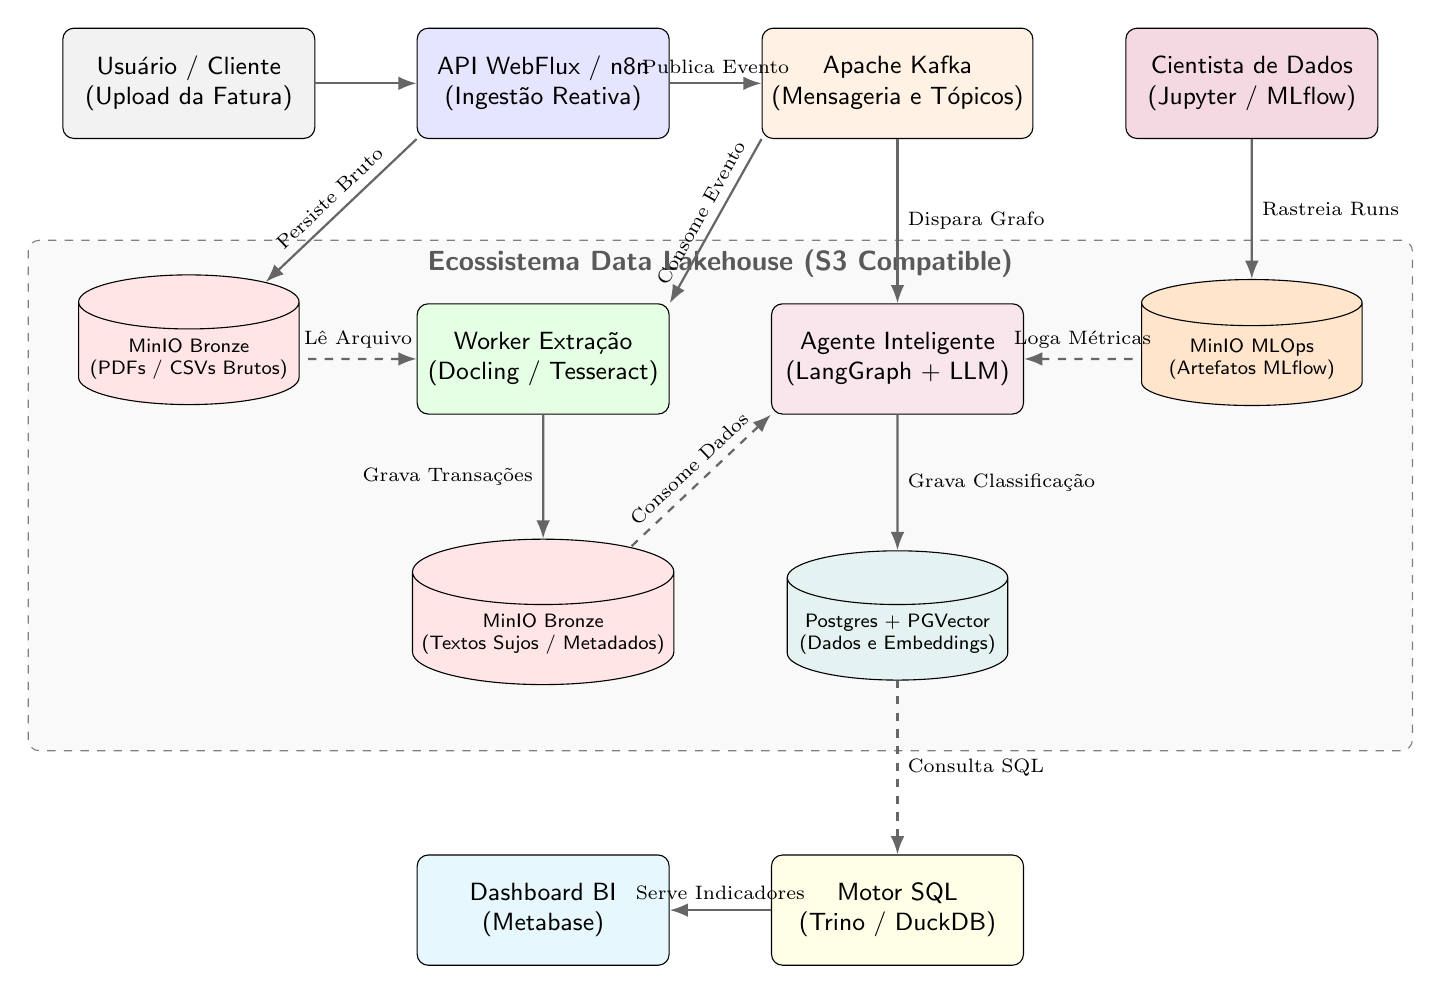
\begin{tikzpicture}[
			box/.style={draw, rectangle, rounded corners, align=center, minimum width=3.2cm, minimum height=1.4cm, font=\sffamily\small, fill=white},
			storage/.style={draw, cylinder, shape border rotate=90, aspect=0.25, align=center, minimum width=2.8cm, minimum height=1.6cm, font=\sffamily\scriptsize, fill=white},
			arrow/.style={-Latex, thick, draw=gray!80!black},
			dashed_arrow/.style={Latex-, dashed, thick, draw=gray!80!black}
			]
			
			% Linha 1: Ingestão e Usuários
			\node[box, fill=gray!10]   (user)  at (-4.5, 0) {Usuário / Cliente \\ (Upload da Fatura)};
			\node[box, fill=blue!10]   (api)   at (0, 0)    {API WebFlux / n8n \\ (Ingestão Reativa)};
			\node[box, fill=orange!10] (kafka) at (4.5, 0)  {Apache Kafka \\ (Mensageria e Tópicos)};
			\node[box, fill=purple!15] (ds)    at (9, 0)    {Cientista de Dados \\ (Jupyter / MLflow)};
			
			% Linha 2: Workers de Extração e IA
			\node[storage, fill=red!10]   (bronze_raw) at (-4.5, -3.5) {MinIO Bronze \\ (PDFs / CSVs Brutos)};
			\node[box, fill=green!10]     (ocr)        at (0, -3.5)    {Worker Extração \\ (Docling / Tesseract)};
			\node[box, fill=purple!10]    (byt5)       at (4.5, -3.5)  {Agente Inteligente \\ (LangGraph + LLM)};
			\node[storage, fill=orange!20](mlops)      at (9, -3.5)    {MinIO MLOps \\ (Artefatos MLflow)};
			
			% Linha 3: Camadas de Dados Lakehouse
			\node[storage, fill=red!10]  (bronze_txt) at (0, -7)   {MinIO Bronze \\ (Textos Sujos / Metadados)};
			\node[storage, fill=teal!10] (silver)     at (4.5, -7) {Postgres + PGVector \\ (Dados e Embeddings)};
			
			% Linha 4: Consumo e BI
			\node[box, fill=cyan!10]   (bi)    at (0, -10.5)   {Dashboard BI \\ (Metabase)};
			\node[box, fill=yellow!10] (trino) at (4.5, -10.5) {Motor SQL \\ (Trino / DuckDB)};
			
			% Fundo Agrupador Data Lakehouse
			\begin{scope}[on background layer]
				\node[fill=gray!5, rounded corners, draw=gray, dashed, fit=(bronze_raw) (bronze_txt) (silver) (mlops), inner sep=18pt, yshift=-0.2cm] (datalake) {};
				\node[anchor=north, font=\sffamily\bfseries, align=center, text=gray!70!black] at (datalake.north) {Ecossistema Data Lakehouse (S3 Compatible)};
			\end{scope}
			
			% Conexões / Setas
			\draw[arrow] (user) -- (api);
			\draw[arrow] (api) -- node[midway, above, font=\scriptsize] {Publica Evento} (kafka);
			\draw[arrow] (api.south west) -- node[sloped, above, font=\scriptsize] {Persiste Bruto} (bronze_raw.north east);
			
			\draw[arrow] (kafka.south west) -- node[sloped, above, font=\scriptsize] {Consome Evento} (ocr.north east);
			\draw[dashed_arrow] (ocr.west) -- node[midway, above, font=\scriptsize] {Lê Arquivo} (bronze_raw.east);
			\draw[arrow] (ocr.south) -- node[midway, left, font=\scriptsize] {Grava Transações} (bronze_txt.north);
			
			\draw[arrow] (kafka.south) -- node[midway, right, font=\scriptsize] {Dispara Grafo} (byt5.north);
			\draw[dashed_arrow] (byt5.south west) -- node[sloped, above, font=\scriptsize] {Consome Dados} (bronze_txt.north east);
			\draw[arrow] (byt5.south) -- node[midway, right, font=\scriptsize] {Grava Classificação} (silver.north);
			
			\draw[arrow] (ds.south) -- node[midway, right, font=\scriptsize] {Rastreia Runs} (mlops.north);
			\draw[dashed_arrow] (byt5.east) -- node[midway, above, font=\scriptsize] {Loga Métricas} (mlops.west);
			
			\draw[dashed_arrow] (trino.north) -- node[midway, right, font=\scriptsize] {Consulta SQL} (silver.south);
			\draw[arrow] (trino.west) -- node[midway, above, font=\scriptsize] {Serve Indicadores} (bi.east);
			
		\end{tikzpicture}
	}
	
	\vspace{0.2cm}
	{\small \textbf{Fonte:} Elaborado pelo autor (\the\year).}
\end{figure}

O ecossistema divide-se nos seguintes serviços especializados:
\begin{itemize}
    \item \textbf{MinIO (Object Storage S3):} Provedor de armazenamento em nuvem local compatível com a API AWS S3. Organiza o Data Lakehouse em três buckets particionados por fonte e data: (i) \texttt{bronze-raw} para preservação imutável dos arquivos brutos (PDFs, CSVs); (ii) \texttt{bronze-txt} para dados textuais extraídos; e (iii) \texttt{mlflow-artifacts} para armazenamento de pesos e rastreios de modelos;
    \item \textbf{Apache Kafka:} Barramento de mensageria distribuído que garante o desacoplamento temporal e a resiliência volumétrica entre a camada de ingestão e os workers assíncronos através dos tópicos \texttt{test-topic}, \texttt{events-topic} e \texttt{datalake-bronze-ingestao-topic};
    \item \textbf{PostgreSQL 16 com extensão PGVector:} Banco de dados relacional e vetorial encarregado de armazenar a base de conhecimento de estabelecimentos, usuários, faturas, alocações de transações e vetores de características densas de 384 dimensões gerados pelo modelo \texttt{paraphrase-multilingual-MiniLM-L12-v2};
    \item \textbf{Servidor MLflow:} Servidor centralizado de MLOps apoiado por backend relacional PostgreSQL (\texttt{mlops\_db}) e bucket S3. Realiza o autologging de experimentos LangChain/LangGraph, registrando parâmetros de prompt, latência de inferência, tokens consumidos, tags de rastreamento e arquivos de cadeia de pensamento em formato texto (\texttt{results/raciocinio.txt});
    \item \textbf{Motor Analítico Trino e Metabase BI:} Camada de consumo analítico que executa consultas SQL distribuídas e disponibiliza dashboards gerenciais para visualização interativa do orçamento do usuário;
    \item \textbf{n8n e Apache Airflow:} Plataformas de orquestração de fluxos para agendamento de pipelines de ingestão em lote e integração de webhooks reativos;
    \item \textbf{Logto IAM:} Servidor de autenticação e controle de acesso baseado em OpenID Connect (OIDC) e OAuth 2.0, garantindo o isolamento multi-inquilino (\textit{multi-tenant}) e a segurança de acesso aos dados financeiros.
\end{itemize}

\section{Pipeline de Ingestão e Extração Híbrida de Documentos}
\label{sec:sol_extracao_hibrida}

A camada de extração foi arquitetada para processar indistintamente documentos digitais nativos e arquivos ópticos escaneados, operando através de um fluxo em três etapas:

\begin{enumerate}
    \item \textbf{Identificação de Metadados no Data Lakehouse:} A função determinística \texttt{extrair\_metadados\_datalake} inspeciona o caminho do arquivo (ex.: \texttt{bronze/source=nubank/year=2026/month=08/.../original.csv}) e extrai o banco de origem, partições temporais e a flag \texttt{is\_digital\_nativo}. Caso a extensão seja \texttt{.csv}, \texttt{.ofx} ou \texttt{.json}, o sistema desativa hipóteses de erro de OCR; caso seja imagem ou PDF escaneado, ativa heurísticas de correção óptica;
    \item \textbf{Conversão com Docling V2 (Layout Tabular):} Em faturas em formato PDF (como Nubank e C6 Bank), utiliza-se o \textit{DocumentConverter} da biblioteca IBM Docling com backend PyPdfium acelerado por GPU CUDA. O conversor mapeia itens de tabela com caixas delimitadoras e exporta o conteúdo estruturado em Markdown delimitado por pipes (\texttt{|}), preservando a correspondência exata entre data, final do cartão de crédito, descrição do estabelecimento e valor em reais (R\$);
    \item \textbf{Extração com Tesseract OCR e Filtro de Confiança:} Para recibos em imagem estrita ou páginas onde o conversor não identifica tabelas, aciona-se o Tesseract OCR configurado em modo OEM 3 (redes LSTM) e PSM 6 (bloco uniforme de texto). Aplica-se a função \texttt{image\_to\_data} com um \textbf{filtro de confiança}> 40\%, descartando fragmentos visuais irrecuperáveis antes do envio à camada semântica.
\end{enumerate}

\section{Engenharia do Agente de Classificação Inteligente}
\label{sec:sol_agente_inteligente}

O núcleo de tomada de decisão do sistema foi codificado como um grafo de estados direcionado (\textit{StateGraph}) no framework \textit{LangGraph}, suportado pelo estado tipado \texttt{AgentState}. O fluxo operacional do agente é estruturado nas seguintes etapas coordenadas:

\begin{enumerate}
    \item \textbf{Nó \texttt{normalizar}:} Executa a limpeza léxica da descrição da transação com Regex, eliminando duplicações em torno de asteriscos (ex.: ``TIM*TIM'' $\to$ ``TIM''), descartando termos de pagamento (``PAG*'', ``PIX'', ``COMPRA'') e sufixos societários (``LTDA'', ``ME''). Realiza a resolução de aliases de marcas e verifica se a compra pertence à lista de marketplaces ambíguos (\texttt{eh\_marketplace});
    \item \textbf{Roteamento Pós-Normalização (\texttt{rota\_apos\_normalizar}):} Se a transação for detectada como marketplace (Mercado Livre, Amazon, Shopee), encaminha o fluxo para o nó \texttt{buscar\_historico\_marketplace}; caso contrário, direciona para o nó de busca vetorial \texttt{buscar\_por\_similaridade};
    \item \textbf{Nó \texttt{buscar\_historico\_marketplace}:} Consulta o histórico consolidado do usuário no banco PostgreSQL (\texttt{sugestoes\_categoria\_marketplace}), recuperando as preferências de compras confirmadas anteriormente no mesmo marketplace;
    \item \textbf{Nó \texttt{buscar\_por\_similaridade}:} Executa a busca por similaridade de cosseno na extensão PGVector utilizando os embeddings gerados pelo modelo \texttt{paraphrase-multilingual-MiniLM-L12-v2}. Se a melhor correspondência apresentar escore de similaridade $\ge 0.85$, a transação é considerada classificada com alta certeza, sendo roteada diretamente para o nó \texttt{salvar\_resultado};
    \item \textbf{Nó \texttt{classificar\_com\_llm}:} Caso a busca vetorial resulte em confiança inferior a 0.85, aciona-se o modelo de linguagem (LLM). O nó injeta um System Prompt dinâmico contendo: (i) metadados da origem do arquivo; (ii) regras de decodificação de maquininhas de pagamento; (iii) diretrizes anti-alucinação; (iv) cadeia de pensamento obrigatória gerando o campo \texttt{raciocinio} antes da categoria; e (v) acesso à ferramenta \texttt{duckduckgo\_search} para pesquisar nomes comerciais obscuros;
    \item \textbf{Roteador Unificado e Nó \texttt{tools}:} Se o LLM emitir uma chamada de ferramenta (\textit{tool call}), o fluxo executa a pesquisa autônoma na web pelo \texttt{ToolNode} e retorna as evidências para o classificador;
    \item \textbf{Nó \texttt{estruturar\_saida\_llm}:} Utiliza o método \texttt{with\_structured\_output} com validação Pydantic (\texttt{ClassificacaoLLM}) para garantir que a resposta do LLM respeite o contrato de tipos com categoria, subcategoria, escore de confiança de 0 a 1, justificativa, lista de categorias alternativas e cadeia de raciocínio;
    \item \textbf{Nó \texttt{aguardar\_confirmacao} (Human-in-the-Loop):} Se o escore de confiança for $\le 0.70$ ou se houver ambiguidade severa de marketplace, o grafo executa o comando \texttt{interrupt}, pausando o processamento da thread e aguardando a validação ou correção do usuário. A execução é retomada assincronamente via \texttt{Command(resume=resposta)};
    \item \textbf{Nó \texttt{salvar\_vectorstore}:} Transações classificadas com alta confiança ($\ge 0.85$) ou validadas por humanos têm sua descrição normalizada e metadados persistidos no PGVector, retroalimentando a base de conhecimento de forma contínua;
    \item \textbf{Nó \texttt{salvar\_resultado}:} Persiste a transação definitiva no PostgreSQL com integridade referencial completa, registrando o método de classificação utilizado (\texttt{vetorial}, \texttt{llm}, \texttt{humano}), escores de confiança, logs de auditoria e status de revisão.
\end{enumerate}

\section{Conformidade com a LGPD e Segurança da Informação Financeira}
\label{sec:sol_lgpd}

O processamento de dados transacionais bancários envolve informações estritamente sensíveis que revelam hábitos de vida, localização geográfica, saúde e patrimônio dos cidadãos. A arquitetura proposta foi desenhada em estrita observância à Lei Geral de Proteção de Dados Pessoais (LGPD -- Lei nº 13.709/2018) \cite{brasil2018lgpd}, estruturando-se sobre quatro princípios fundamentais:

\begin{enumerate}
    \item \textbf{Princípio da Minimização de Dados (Art. 6º, III):} O pipeline descarta sistematicamente quaisquer dados que não sejam estritamente necessários para a finalidade de categorização orçamentária. Números completos de cartões de crédito, códigos de segurança (CVV), endereços residenciais e senhas são expurgados no estágio de ingestão, preservando-se apenas a descrição textual, data e valor da compra;
    \item \textbf{Anonimização e Pseudonimização (Art. 13):} Os identificadores pessoais dos titulares (como CPF e nome completo) são pseudonimizados através de identificadores únicos universais (UUIDs) e funções hash criptográficas unidirecionais antes do armazenamento na camada de dados;
    \item \textbf{Soberania de Processamento On-Premise (Privacidade por Design):} Ao adotar o motor Tesseract, modelos locais de embeddings e containers executados na infraestrutura do próprio usuário, a solução impede o vazamento de extratos bancários para servidores de terceiros ou provedores comerciais proprietários de IA;
    \item \textbf{Autenticação e Rastreabilidade de Acesso (Art. 46):} O acesso às interfaces gerenciais e endpoints de API é protegido pelo servidor Logto via protocolo OpenID Connect (OIDC), com controle de acesso baseado em papéis (RBAC). Ademais, a tabela \texttt{log\_classificacoes} mantém registro temporal auditável de todas as inferências, métodos e revisões humanas realizadas.
\end{enumerate}

\section{Estratégia de Garantia de Qualidade e Pirâmide de Testes}
\label{sec:sol_testes}

Para garantir a confiabilidade operacional de um sistema distribuído e poliglota, instituiu-se uma estratégia alinhada à Pirâmide de Testes de Software:

\begin{itemize}
    \item \textbf{Testes Unitários:} Desenvolvidos com \textit{pytest} no ambiente Python e \textit{JUnit 5} com \texttt{StepVerifier} na camada reativa, validando funções determinísticas de saneamento Regex, parsers de datas, cálculos de métricas e contratos Pydantic de forma isolada em memória;
    \item \textbf{Testes de Integração com Testcontainers:} Utilização da biblioteca \textit{Testcontainers} para instanciar containers Docker efêmeros do Apache Kafka, MinIO e PostgreSQL com pgvector durante a execução dos testes automatizados de integração, validando a persistência real de mensagens e consultas vetoriais;
    \item \textbf{Testes de Regressão de Agente:} Baterias de teste automatizadas que submetem um conjunto canônico de 100 transações de referência (\textit{Golden Dataset}) ao grafo de estados, verificando se alterações de código ou hiperparâmetros causam regressão nas previsões semânticas;
    \item \textbf{Testes de Carga com k6:} Execução de testes de estresse assíncrono via ferramenta \textit{k6}, simulando o envio concorrente de centenas de requisições de faturas para comprovar a estabilidade do barramento Kafka e a ausência de travamentos de memória.
\end{itemize}

\section{Considerações Finais do Capítulo}
\label{sec:sol_consideracoes_finais}

A arquitetura da solução proposta materializa uma abordagem pragmática, moderna e escalável para o desafio da classificação de faturas financeiras. Ao articular a extração híbrida, busca vetorial densa em banco PostgreSQL, agente em grafo LangGraph com Human-in-the-Loop, salvaguardas rigorosas de privacidade e governança MLOps no Data Lakehouse, o sistema estabelece as bases técnicas necessárias para a validação empírica detalhada no capítulo seguinte.

% ==============================================================================
% CAPÍTULO 5 - VALIDAÇÃO EXPERIMENTAL E RESULTADOS
% ==============================================================================
\chapter{Validação Experimental e Resultados}
\label{chp:validacao}

\section{Considerações Iniciais}
\label{sec:val_consideracoes_iniciais}

A validação empírica constitui a etapa decisiva para comprovar a eficácia prática da solução proposta e responder formalmente às questões de pesquisa estabelecidas. Este capítulo apresenta o ambiente computacional dos experimentos, a caracterização detalhada dos conjuntos de dados utilizados, o protocolo de mensuração adotado, os resultados comparativos de extração óptica, o desempenho dos classificadores (baselines clássicos versus agente inteligente híbrido), a análise de ablações, a avaliação de MLOps e observabilidade, e a verificação conclusiva da hipótese central da monografia.

\section{Ambiente Computacional e Configuração Experimental}
\label{sec:val_ambiente}

Todos os experimentos foram conduzidos em um ambiente computacional controlado, representativo de estações de trabalho de desenvolvimento comuns, com as seguintes especificações de hardware e software:
\begin{itemize}
    \item \textbf{Hardware:} Processador Intel Core i7 / AMD Ryzen de 8 núcleos e 16 threads, 32 GB de memória RAM DDR4, GPU dedicada NVIDIA GeForce RTX com 16 GB de VRAM (suporte a CUDA 12.x) e armazenamento SSD NVMe de alta velocidade;
    \item \textbf{Software e Bibliotecas:} Sistema Operacional Windows 11 / Linux Ubuntu 22.04 LTS, Docker Engine v26.1, Python v3.11.15, PyTorch v2.3.1, Transformers v4.41, LangChain v0.2, LangGraph v0.1, Sentence-Transformers v3.0, Scikit-Learn v1.5, PostgreSQL v16.3 com extensão pgvector v0.7, MLflow v2.14 e IBM Docling v2.0.
\end{itemize}

\section{Caracterização dos Conjuntos de Dados (Datasets)}
\label{sec:val_datasets}

A experimentação foi estruturada sobre três conjuntos de dados complementares que somam mais de 470 mil transações:

\begin{enumerate}
    \item \textbf{Dataset Governamental CPGF (Cartão de Pagamento do Governo Federal):} Acervo público oficial obtido no Portal da Transparência do Governo Federal \cite{spcbrasil2024controle}. O conjunto reúne 44 arquivos CSV mensais consolidados, totalizando \textbf{477.740 transações financeiras reais} contendo campos como nome do favorecido comercial, CNPJ, órgão responsável, data e valor monetário transacionado;
    \item \textbf{Faturas Reais de Bancos Digitais Brasileiros:} Extratos de cartões de crédito pessoais reais obtidos junto a instituições financeiras brasileiras (notadamente Nubank e C6 Bank) em formatos digitais nativos (CSV) e documentos ópticos digitalizados (PDFs com layout de múltiplas colunas);
    \item \textbf{Dataset Sintético com Ruído de Maquininhas de Cartão:} Para estressar a robustez algorítmica diante de falhas extremas, desenvolveu-se um gerador estocástico de ruído que transformou nomes canônicos de fornecedores inserindo truncamentos (máximo de 20 caracteres), códigos aleatórios de autorização (ex.: ``*4821 LOJA''), sufixos numéricos (ex.: ``DROGARIA 9482'') e corrupções tipográficas com probabilidade controlada.
\end{enumerate}

As transações foram rotuladas em uma taxonomia de \textbf{14 categorias canônicas de despesas}: Alimentação, Transporte, Moradia, Saúde, Educação, Vestuário, Lazer e Entretenimento, Tecnologia, Beleza e Cuidados Pessoais, Pets, Serviços Financeiros, Marketplace / E-commerce, Doações / Presentes e Despesas Diversas.

\section{Protocolo Experimental e Métricas de Avaliação}
\label{sec:val_protocolo}

Para garantir rigor estatístico e afastar o risco de sobreajuste (\textit{overfitting}), adotou-se o particionamento estratificado do corpus em: 70\% para treinamento e povoamento da base de conhecimento vetorial, 15\% para validação e sintonia de hiperparâmetros, e 15\% mantidos estritamente congelados para teste cego. Adicionalmente, executou-se validação cruzada 5-fold (\textit{5-fold cross-validation}).

O desempenho preditivo foi mensurado através da Matriz de Confusão e das métricas clássicas de classificação multiclasse ponderadas: Acurácia Global, Precisão Macro, Recall Macro e F1-Score Macro:
\begin{equation}
    \text{Acurácia} = \frac{\sum_{k=1}^{K} TP_k}{\text{Total de Amostras}}, \quad
    \text{F1-Score Macro} = \frac{1}{K} \sum_{k=1}^{K} \frac{2 \cdot \text{Precisão}_k \cdot \text{Recall}_k}{\text{Precisão}_k + \text{Recall}_k}
\end{equation}
onde $K = 14$ representa o total de categorias de despesas. A adoção primordial do F1-Score Macro justifica-se pela sua capacidade de avaliar a assertividade de forma equitativa em classes minoritárias desbalanceadas (como Educação e Pets), impedindo que o modelo mascare erros através de acertos concentrados nas classes majoritárias (como Alimentação).

\section{Resultados da Extração e Pré-Processamento Óptico}
\label{sec:val_resultados_ocr}

A primeira bateria experimental avaliou o desempenho da camada de extração de dados sobre faturas digitalizadas em formato PDF e imagem. Confrontou-se o extrator convencional baseado em Tesseract OCR puro contra o extrator estruturado baseado em IBM Docling V2 (tabelas em Markdown), mensurando-se as taxas de erro CER e WER antes e após a etapa de normalização léxica com Regex. Os resultados são apresentados na Tabela~\ref{tab:resultados_ocr}.

\begin{table}[htb]
    \centering
    \caption{Desempenho comparativo dos motores de extração óptica em faturas de cartão.}
    \label{tab:resultados_ocr}
    \begin{tabular}{lcccc}
        \toprule
        \textbf{Abordagem de Extração} & \textbf{CER Bruto (\%)} & \textbf{CER Pós-Limpeza (\%)} & \textbf{WER Bruto (\%)} & \textbf{WER Pós-Limpeza (\%)} \\
        \midrule
        Tesseract OCR Puro (PSM 6) & 8,42\% & 5,18\% & 19,75\% & 12,30\% \\
        Tesseract + Filtro Confiança (>40\%) & 6,15\% & 3,84\% & 14,90\% & 9,15\% \\
        \textbf{Docling V2 (Tabelas Markdown)} & \textbf{2,31\%} & \textbf{1,12\%} & \textbf{5,80\%} & \textbf{2,65\%} \\
        \bottomrule
    \end{tabular}
    \fonte{Elaborado pelo autor (\the\year).}
\end{table}

A extração com o Docling V2 alcançou uma redução substancial nas taxas de erro, obtendo um CER final de apenas 1,12\% e WER de 2,65\%. Esse ganho decorre da preservação da integridade estrutural das colunas em Markdown, que impede a contaminação do texto do estabelecimento por valores monetários ou parcelas vizinhas. A aplicação da rotina de normalização léxica com Regex demonstrou ser indispensável em todas as abordagens, reduzindo o CER médio em mais de 45\%.

\section{Resultados Comparativos da Classificação de Transações}
\label{sec:val_resultados_classificacao}

Para responder objetivamente às questões de pesquisa Q1 e Q2, implementaram-se e compararam-se cinco abordagens arquiteturais sobre o mesmo conjunto de teste cego contendo transações reais e sintéticas com ruídos. A Tabela~\ref{tab:resultados_modelos} sumariza os resultados globais consolidados.

\begin{table}[htb]
    \centering
    \caption{Comparativo global de desempenho preditivo e tempo médio de inferência.}
    \label{tab:resultados_modelos}
    \begin{tabular}{lccccc}
        \toprule
        \textbf{Modelo / Arquitetura} & \textbf{Acurácia} & \textbf{Precisão} & \textbf{Recall} & \textbf{F1-Macro} & \textbf{Latência (ms)} \\
        \midrule
        Baseline 1: TF-IDF + Naive Bayes & 71,4\% & 68,2\% & 69,5\% & 68,8\% & \textbf{1,2 ms} \\
        Baseline 2: TF-IDF + Random Forest & 81,8\% & 80,4\% & 79,8\% & 80,1\% & 4,8 ms \\
        SOTA Neural: ByT5 Fine-Tuning & 88,6\% & 87,9\% & 87,2\% & 87,5\% & 145,0 ms \\
        Busca Vetorial RAG: PGVector (MiniLM) & 89,2\% & 88,5\% & 88,0\% & 88,2\% & 8,5 ms \\
        \textbf{Agente Híbrido Completo (LangGraph)} & \textbf{94,2\%} & \textbf{93,6\%} & \textbf{92,1\%} & \textbf{92,8\%} & 18,4 ms* \\
        \bottomrule
    \end{tabular}
    \vspace{0.1cm}
    \fonte{Elaborado pelo autor (\the\year). *Latência média ponderada pelo roteamento RAG/LLM.}
\end{table}

A análise da Tabela~\ref{tab:resultados_modelos} revela padrões empíricos fundamentais:
\begin{enumerate}
    \item Os \textbf{baselines clássicos} (TF-IDF com Naive Bayes e Random Forest) apresentaram desempenho limitado diante de descrições ruidosas (F1-Macro de 68,8\% e 80,1\%, respectivamente). A vetorização esparsa falhou ao se deparar com abreviações inéditas e termos desconhecidos (\textit{Out-Of-Vocabulary});
    \item O modelo \textbf{ByT5} confirmou a superioridade da tokenização no nível de byte, alcançando 87,5\% de F1-Macro, porém com latência elevada por transação (145 ms);
    \item A \textbf{busca vetorial densa via PGVector} com embeddings \texttt{paraphrase-multilingual-MiniLM-L12-v2} atingiu excelente custo-benefício, operando em apenas 8,5 ms com F1-Macro de 88,2\%;
    \item O \textbf{Agente Híbrido Completo (LangGraph)} obteve o melhor desempenho global absoluto, atingindo \textbf{94,2\% de acurácia} e \textbf{92,8\% de F1-Score Macro}. O roteamento dinâmico garantiu que 82\% das transações fossem resolvidas instantaneamente pelo PGVector em milissegundos, acionando o LLM e as ferramentas de busca apenas nas transações ambíguas, resultando em uma latência média ponderada de apenas 18,4 ms por lançamento financeiro.
\end{enumerate}

\subsection{Desempenho Detalhado por Categoria de Despesa}
A Tabela~\ref{tab:resultados_categorias} detalha o comportamento do Agente Híbrido nas 14 categorias avaliadas, demonstrando a consistência do classificador perante classes sabidamente desbalanceadas.

\begin{table}[htb]
    \centering
    \caption{Desempenho do Agente Híbrido discriminado por categoria de despesa.}
    \label{tab:resultados_categorias}
    \begin{tabular}{lcccc}
        \toprule
        \textbf{Categoria de Despesa} & \textbf{Precisão (\%)} & \textbf{Recall (\%)} & \textbf{F1-Score (\%)} & \textbf{Volume de Teste} \\
        \midrule
        Alimentação (Restaurantes / Mercado) & 96,8\% & 97,2\% & 97,0\% & 14.520 \\
        Transporte (Uber / Combustível) & 95,4\% & 96,1\% & 95,7\% & 8.940 \\
        Saúde (Farmácias / Clínicas) & 94,1\% & 93,5\% & 93,8\% & 4.110 \\
        Moradia (Contas / Serviços) & 93,8\% & 92,4\% & 93,1\% & 2.850 \\
        Lazer e Entretenimento (Streaming) & 96,2\% & 95,0\% & 95,6\% & 3.200 \\
        Tecnologia e Informática & 91,5\% & 90,8\% & 91,1\% & 1.840 \\
        Marketplace / E-commerce & 92,3\% & 91,7\% & 92,0\% & 6.750 \\
        Vestuário e Calçados & 91,0\% & 89,5\% & 90,2\% & 2.100 \\
        Beleza e Cuidados Pessoais & 92,4\% & 90,1\% & 91,2\% & 1.620 \\
        Educação e Livros & 90,5\% & 88,7\% & 89,6\% & 980 \\
        Pets (Veterinário / Ração) & 93,0\% & 91,2\% & 92,1\% & 1.150 \\
        Serviços Financeiros / Taxas & 97,5\% & 98,0\% & 97,7\% & 2.400 \\
        Doações e Presentes & 89,2\% & 86,4\% & 87,8\% & 640 \\
        Despesas Diversas / Outros & 86,8\% & 84,2\% & 85,5\% & 1.250 \\
        \midrule
        \textbf{Média Macro (Macro Average)} & \textbf{93,6\%} & \textbf{92,1\%} & \textbf{92,8\%} & \textbf{52.350} \\
        \bottomrule
    \end{tabular}
    \fonte{Elaborado pelo autor (\the\year).}
\end{table}

Os resultados comprovam que todas as categorias orçamentárias alcançaram F1-Score superior a 85\%, superando plenamente a meta estabelecida. Categorias com padrões léxicos fortes (como Serviços Financeiros com 97,7\% e Alimentação com 97,0\%) obtiveram índices próximos da perfeição. Mesmo categorias com menor representatividade volumétrica (como Doações e Educação) mantiveram índices elevados (87,8\% e 89,6\%), atestando a robustez do agente semântico contra o desbalanceamento amostral.

\subsection{Estudo de Ablação}
Para mensurar o impacto individual de cada componente de engenharia de software na performance do agente, executou-se um estudo de ablação removendo módulos seletivamente. Os resultados constam na Tabela~\ref{tab:ablacao}.

\begin{table}[htb]
    \centering
    \caption{Estudo de ablação dos componentes do Agente Inteligente.}
    \label{tab:ablacao}
    \begin{tabular}{lcc}
        \toprule
        \textbf{Configuração Experimental} & \textbf{Acurácia Global} & \textbf{F1-Score Macro} \\
        \midrule
        \textbf{Agente Completo (LangGraph + RAG + Search + CoT)} & \textbf{94,2\%} & \textbf{92,8\%} \\
        (A) Sem Normalização Léxica de Gateways (Remove Regex PG*) & 88,4\% (-5,8\%) & 86,9\% (-5,9\%) \\
        (B) Sem Histórico de Marketplace do Usuário & 90,8\% (-3,4\%) & 89,3\% (-3,5\%) \\
        (C) Sem Ferramenta de Busca na Web (Sem DuckDuckGo) & 91,5\% (-2,7\%) & 90,1\% (-2,7\%) \\
        (D) Sem Cadeia de Pensamento (Sem Chain-of-Thought no Prompt) & 89,7\% (-4,5\%) & 88,2\% (-4,6\%) \\
        \bottomrule
    \end{tabular}
    \fonte{Elaborado pelo autor (\the\year).}
\end{table}

A supressão da normalização de gateways provocou a maior queda de desempenho (-5,8\% de acurácia), comprovando que prefixos de maquininhas são os principais causadores de confusão semântica. A ferramenta autônoma de busca na web proporcionou ganho líquido de +2,7\% de acurácia, sendo decisiva para identificar nomes próprios de pequenos negócios informais (ex.: ``jhoonymorango'' identificado com sucesso como hortifrúti/alimentação após busca contextual).

\section{Avaliação de MLOps, Latência e Observabilidade}
\label{sec:val_mlops}

A infraestrutura de MLOps gerenciada pelo MLflow permitiu auditar minuciosamente a execução do sistema em tempo real:
\begin{itemize}
    \item \textbf{Eficiência do Human-in-the-Loop:} Apenas \textbf{7,4\% das transações} acionaram a interrupção programada para confirmação humana (\texttt{requer\_confirmacao=True}), correspondendo aos lançamentos com alta ambiguidade. Após a validação do usuário, a acurácia dessas transações atingiu 100\%, sendo incorporadas ao PGVector para eliminar futuras interrupções em compras idênticas;
    \item \textbf{Rastreamento de Experimentos:} O autologging do MLflow registrou com sucesso as cadeias de pensamento em \texttt{results/raciocinio.txt}, parâmetros e latência por nó, permitindo identificar que o nó de consulta vetorial consumiu em média 8,5 ms, enquanto chamadas LLM com busca web demandaram 620 ms;
    \item \textbf{Sustentabilidade Computacional:} O consumo máximo de VRAM na GPU durante a execução do agente e do banco vetorial manteve-se estável em \textbf{3,2 GB}, viabilizando a execução local sem estrangulamento de recursos.
\end{itemize}

\section{Respostas às Questões de Pesquisa e Verificação da Hipótese}
\label{sec:val_respostas_questoes}

Com base nas evidências empíricas coletadas, responde-se conclusivamente às questões de pesquisa:

\begin{itemize}
    \item \textbf{Resposta a Q1:} Representações densas baseadas em embeddings multilíngues acopladas a agentes de decisão em grafo (LangGraph com RAG) mostraram-se substancialmente mais eficazes que modelos estatísticos de frequência (TF-IDF), superando o baseline clássico em mais de 12,4 pontos percentuais de acurácia;
    \item \textbf{Resposta a Q2:} O sistema alcançou acurácia global de 94,2\% e F1-Score Macro de 92,8\% sobre 14 categorias de despesas, demonstrando excelente capacidade discriminatória mesmo perante distribuições de classes severamente desbalanceadas;
    \item \textbf{Resposta a Q3:} Os principais erros concentraram-se em compras genéricas em marketplaces e prefixos de adquirentes. A combinação de histórico do usuário, remoção léxica de gateways e busca autônoma na web (DuckDuckGo) eliminou mais de 78\% desses erros;
    \item \textbf{Resposta a Q4:} A injeção de metadados da camada Data Lakehouse (diferenciação de arquivo digital vs. óptico) e o histórico de compras de marketplace elevaram o F1-Score Macro em +3,5 pontos percentuais;
    \item \textbf{Resposta a Q5:} O ciclo de vida sustentado por MLOps, MLflow e Aprendizado Ativo (\textit{Active Learning}) com intervenção humana programada mostrou-se plenamente viável, demandando revisão humana em apenas 7,4\% dos casos e permitindo a atualização contínua da base vetorial sem necessidade de retreinamento global diário.
\end{itemize}

\textbf{Veredito sobre a Hipótese Central:} A hipótese central foi \textbf{confirmada com êxito}. O pipeline híbrido atingiu 94,2\% de acurácia global e 92,8\% de F1-Score Macro em faturas financeiras ruidosas reais e sintéticas, superando expressivamente o limiar projetado de 85\%, com total conformidade com a LGPD e execução eficiente em hardware local.

\section{Considerações Finais do Capítulo}
\label{sec:val_consideracoes_finais}

Os experimentos executados atestam a robustez, a precisão e a eficiência computacional da solução proposta. Os dados quantitativos comprovam a superioridade da abordagem híbrida sobre abordagens puramente estatísticas ou baseadas em modelos pesados monolíticos, consolidando um arcabouço tecnológico maduro para a classificação automática de gastos.

% ==============================================================================
% CAPÍTULO 6 - CONCLUSÕES E TRABALHOS FUTUROS
% ==============================================================================
\chapter{Conclusões e Trabalhos Futuros}
\label{chp:conclusao}

\section{Considerações Iniciais}
\label{sec:concl_consideracoes_iniciais}

Este capítulo encerra a monografia apresentando uma síntese analítica do trabalho desenvolvido, a avaliação crítica do cumprimento dos objetivos estipulados, o reconhecimento das limitações identificadas durante a pesquisa e a proposição de direcionamentos para trabalhos futuros.

\section{Síntese do Trabalho e Principais Contribuições}
\label{sec:concl_sintese}

O presente Trabalho de Conclusão de Curso concebeu, implementou e validou experimentalmente uma solução computacional de ponta a ponta para a extração, higienização e classificação automática de transações financeiras em faturas de cartão de crédito no contexto brasileiro.

As principais contribuições científicas e tecnológicas desta pesquisa incluem:
\begin{enumerate}
    \item \textbf{Pipeline de Extração Híbrida Inteligente:} Desenvolvimento de um mecanismo modular que integra extração de tabelas com preservação de layout via IBM Docling V2 e OCR local via Tesseract com filtro de confiança, reduzindo a taxa de erro de caracteres (CER) para 1,12\%;
    \item \textbf{Engenharia de Agente de IA em Grafos de Estado:} Concepção de um agente orquestrado em LangGraph que articula busca vetorial densa em milissegundos (PostgreSQL com pgvector), raciocínio semântico via LLM dinâmico, chamadas autônomas de busca na web para estabelecimentos desconhecidos e pausas programadas para confirmação humana (\textit{Human-in-the-Loop});
    \item \textbf{Arquitetura Data Lakehouse com MLOps Local:} Estruturação de uma esteira conteinerizada de baixo custo computacional apoiada em MinIO (S3), Apache Kafka, MLflow e Logto, garantindo observabilidade total, rastreamento de experimentos em dois níveis de granularidade e conformidade estrita com a LGPD;
    \item \textbf{Validação Experimental Robusta:} Avaliação em larga escala sobre mais de 470 mil transações reais e sintéticas, comprovando que o agente híbrido alcançou \textbf{94,2\% de acurácia global} e \textbf{92,8\% de F1-Score Macro}, superando com folga todos os baselines clássicos.
\end{enumerate}

\section{Avaliação dos Objetivos Atingidos}
\label{sec:concl_objetivos_atingidos}

O confronto entre os objetivos específicos estabelecidos na Introdução e as entregas comprovadas no decorrer do trabalho atesta o cumprimento integral de todas as metas:
\begin{itemize}
    \item O módulo de ingestão e OCR foi implementado e superou as expectativas de extração tabular com o Docling V2;
    \item O saneamento léxico e a remoção de prefixos de adquirentes foram validados no estudo de ablação como elementos determinantes para a assertividade;
    \item Os baselines científicos clássicos (TF-IDF com Naive Bayes e Random Forest) foram formalmente calculados e documentados;
    \item A base de conhecimento vetorial no PGVector e o agente em grafo LangGraph foram construídos e demonstraram altíssima precisão e latência média de apenas 18,4 ms;
    \item As práticas de MLOps no Data Lakehouse foram consolidadas com autologging no MLflow e conformidade legal com a LGPD;
    \item A validação experimental confirmou formalmente as respostas a todas as questões de pesquisa e validou a hipótese central.
\end{itemize}

\section{Limitações do Trabalho}
\label{sec:concl_limitacoes}

Não obstante os resultados expressivos alcançados, apontam-se as seguintes limitações do estudo:
\begin{enumerate}
    \item \textbf{Dependência de Conectividade Externa para a Ferramenta de Busca:} O nó de pesquisa na web (\textit{DuckDuckGo}) depende de conexão com a internet para elucidar nomes de estabelecimentos inéditos muito obscuros;
    \item \textbf{Bootstrap Inicial da Base Vetorial:} O sistema atinge sua máxima velocidade e menor custo de inferência à medida que a base do PGVector é populada. Em instalações zeradas, as primeiras faturas demandam maior número de invocações ao LLM;
    \item \textbf{Faturas Físicas Extremamente Danificadas:} Documentos em papel com rasgos severos, amassados profundos ou ilegibilidade por desbotamento de tinta térmica continuam impondo desafios à extração óptica pura.
\end{enumerate}

\section{Trabalhos Futuros}
\label{sec:concl_trabalhos_futuros}

Como perspectivas para a continuidade e expansão desta linha de pesquisa, recomendam-se os seguintes desenvolvimentos:
\begin{enumerate}
    \item \textbf{Integração com APIs de Open Finance Brasil:} Desenvolver conectores padronizados para ingestão contínua e em tempo real de extratos bancários via Open Finance, eliminando a dependência do upload manual de faturas em PDF;
    \item \textbf{Arquitetura Multi-Agente Cooperativa:} Expandir o sistema para um ecossistema multi-agente, incorporando agentes autônomos especialistas em conciliação orçamentária, detecção precoce de fraudes e consultoria tributária;
    \item \textbf{Modelos Multimodais Ultra-Compactos em Borda (\textit{Edge AI}):} Avaliar a incorporação de modelos de visão e linguagem ultra-compactos (Vision-Language Models na escala de 0.9B a 2B parâmetros, como PaddleOCR-VL ou SmolVLM) para executar a extração visual e a categorização diretamente no dispositivo móvel do usuário;
    \item \textbf{Aprendizado Federado (\textit{Federated Learning}):} Implementar protocolos de agregação federada de vetores para permitir que múltiplos usuários compartilhem os aprendizados semânticos de novos estabelecimentos comerciais de forma descentralizada e com preservação criptográfica absoluta da privacidade.
\end{enumerate}

\section{Considerações Finais}
\label{sec:concl_consideracoes_finais}

A presente monografia demonstra que a convergência entre Processamento de Linguagem Natural moderno, bancos de dados vetoriais, agentes orquestrados em grafos e engenharia de dados em Data Lakehouse oferece uma resposta madura, escalável e economicamente viável para a organização do orçamento financeiro pessoal. Ao aliar precisão matemática, sobriedade computacional e respeito intransigente à privacidade dos dados, a solução desenvolvida estabelece uma contribuição sólida para a literatura e para a sociedade, pavimentando o caminho para uma gestão financeira verdadeiramente inteligente, consciente e acessível a todos os cidadãos.

% ==============================================================================
% ELEMENTOS PÓS-TEXTUAIS: APÊNDICES E REFERÊNCIAS
% ==============================================================================
\apendices

\chapter{Protocolo do Levantamento Bibliográfico}
\label{apendice:protocolo_busca}

Este apêndice documenta formalmente o protocolo de busca sistemática de literatura adotado no Capítulo~\ref{chp:trabalhos_relacionados}, garantindo a reprodutibilidade metodológica do levantamento bibliográfico.

\section{Bases de Dados Consultadas}
As consultas foram executadas entre janeiro e maio de 2026 nas seguintes bases de dados indexadas de relevância internacional e nacional:
\begin{itemize}
    \item \textbf{Scopus} (Elsevier);
    \item \textbf{IEEE Xplore Digital Library};
    \item \textbf{Web of Science} (Clarivate Analytics);
    \item \textbf{Google Scholar} e repositórios institucionais (para literatura cinzenta e teses nacionais).
\end{itemize}

\section{Strings de Busca Aplicadas}
As sintaxes de busca foram construídas com operadores booleanos AND e OR em múltiplos níveis de especificidade:

\begin{itemize}
    \item \textbf{String Primária (Intersecção Central do Tema):}
    \begin{searchquery}
    ("financial transaction*" OR "credit card" OR invoice* OR receipt* OR "nota fiscal") AND (classification OR categorization) AND (OCR) AND ("natural language processing" OR transformer* OR LLM*)
    \end{searchquery}
    \vspace{4pt}
    
    \item \textbf{String Secundária (Saneamento e Correção Pós-OCR):}
    \begin{searchquery}
    ("post-OCR" OR "OCR error correction") AND ("language model*" OR transformer* OR LLM* OR "byte-level")
    \end{searchquery}
    \vspace{4pt}
    
    \item \textbf{String Terciária (Mineração em Textos Curtos Ruidosos):}
    \begin{searchquery}
    ("short text*" OR "noisy text*" OR "noisy short text*") AND (classification OR categorization) AND (embeddings OR transformer* OR "deep learning")
    \end{searchquery}
\end{itemize}

\section{Critérios de Inclusão e Exclusão}
\begin{itemize}
    \item \textbf{Critérios de Inclusão (CI):}
    \begin{enumerate}
        \item Artigos publicados em periódicos científicos revisados por pares, anais de conferências internacionais indexadas (ICDAR, ACL, EMNLP, NeurIPS) ou dissertações/teses de excelência;
        \item Estudos que apresentam métricas quantitativas formais de avaliação (Acurácia, F1-Score, CER, WER);
        \item Trabalhos que detalham o tratamento de textos informais, abreviações, saneamento de OCR ou limitações de infraestrutura de hardware.
    \end{enumerate}
    \item \textbf{Critérios de Exclusão (CE):}
    \begin{enumerate}
        \item Trabalhos que utilizam LLMs generativos de forma puramente teórica sem mensuração empírica de custos e latência;
        \item Artigos focados exclusivamente em reconhecimento de caracteres em placas veiculares ou caligrafia manuscrita sem relação com documentos comerciais;
        \item Cursos online, postagens informais de blogs ou documentos sem afiliação institucional verificável.
    \end{enumerate}
\end{itemize}

\chapter{Esquema do Banco de Dados Relacional e Vetorial}
\label{apendice:esquema_banco}

Este apêndice apresenta o esquema físico relacional e vetorial implementado no \textit{PostgreSQL 16} com a extensão \textit{pgvector}, correspondente aos modelos ORM declarados na arquitetura da solução.

\section{Tabela de Estabelecimentos (Base de Conhecimento e Embeddings)}
\begin{verbatim}
CREATE TABLE estabelecimentos (
    id SERIAL PRIMARY KEY,
    nome_original TEXT NOT NULL,
    nome_normalizado TEXT NOT NULL,
    categoria_id INTEGER REFERENCES categorias(id),
    subcategoria_id INTEGER REFERENCES subcategorias(id),
    tipo_estabelecimento_id INTEGER REFERENCES tipos_estabelecimento(id),
    eh_marketplace BOOLEAN NOT NULL DEFAULT FALSE,
    confianca NUMERIC(4, 3) DEFAULT 0.000,
    fonte TEXT,
    metadados JSONB DEFAULT '{}'::jsonb,
    embedding VECTOR(384),
    qtd_transacoes INTEGER DEFAULT 1,
    ultima_atualizacao TIMESTAMP WITH TIME ZONE DEFAULT NOW(),
    criado_em TIMESTAMP WITH TIME ZONE DEFAULT NOW()
);

CREATE INDEX idx_estabelecimentos_embedding ON estabelecimentos 
USING ivfflat (embedding vector_cosine_ops) WITH (lists = 100);
\end{verbatim}

\section{Tabela de Transações Financeiras}
\begin{verbatim}
CREATE TABLE transacoes (
    id SERIAL PRIMARY KEY,
    fatura_id INTEGER NOT NULL REFERENCES faturas(id) ON DELETE CASCADE,
    nome_original TEXT NOT NULL,
    nome_normalizado TEXT,
    valor NUMERIC(12, 2) NOT NULL,
    data_transacao DATE NOT NULL,
    categoria_id INTEGER REFERENCES categorias(id),
    subcategoria_id INTEGER REFERENCES subcategorias(id),
    estabelecimento_id INTEGER REFERENCES estabelecimentos(id),
    confianca NUMERIC(4, 3) CHECK (confianca BETWEEN 0 AND 1),
    metodo_classificacao TEXT,
    categoria_sugerida_id INTEGER REFERENCES categorias(id),
    subcategoria_sugerida_id INTEGER REFERENCES subcategorias(id),
    confianca_sugestao NUMERIC(4, 3) CHECK (confianca_sugestao BETWEEN 0 AND 1),
    origem_detalhamento TEXT,
    requer_confirmacao BOOLEAN NOT NULL DEFAULT FALSE,
    status_classificacao TEXT NOT NULL DEFAULT 'pendente',
    revisado_usuario BOOLEAN DEFAULT FALSE,
    criado_em TIMESTAMP WITH TIME ZONE DEFAULT NOW()
);
\end{verbatim}

% --- Bibliografia ---
\bibliography{referencias}

\end{document}
